%-----------------------------------------------
%  Engineer's & Master's Thesis Template
%  Copyleft by Artur M. Brodzki & Piotr Woźniak
%  Warsaw University of Technology, 2019-2022
%-----------------------------------------------

\documentclass[
    bindingoffset=5mm,  % Binding offset
    footnoteindent=3mm, % Footnote indent
    hyphenation=true    % Hyphenation turn on/off
]{src/wut-thesis}

\usepackage{tikz}
\usetikzlibrary{shapes.geometric, arrows, fit, backgrounds}
\usepackage{listings, src/listings-rust}
\usepackage{pgf-umlsd}
\usepackage{algorithm}
\usepackage{algpseudocode}
\usepackage{enumitem}
\usepackage{courier}
\usepackage{svg}
\usepackage{tabularx}
\usepackage{subfig}
\captionsetup[subfigure]{labelformat=empty}

\newcommand{\newthreadShift}[4][gray!30]{
  \newinst[#4]{#2}{#3}
  \stepcounter{threadnum}
  \node[below of=inst\theinstnum,node distance=0.8cm] (thread\thethreadnum) {};
  \tikzstyle{threadcolor\thethreadnum}=[fill=#1]
  \tikzstyle{instcolor#2}=[fill=#1]
}
\renewcommand\lstlistlistingname{List of Listings}

\lstset{
    escapeinside={<@}{@>},numbers=left,captionpos=b,
    basicstyle=\footnotesize\tt,breaklines=true
}
\graphicspath{{tex/img/}} % Katalog z obrazkami.
\addbibresource{bibliografia.bib} % Plik .bib z bibliografią

%-------------------------------------------------------------
% Wybór wydziału:
%  \facultyeiti: Wydział Elektroniki i Technik Informacyjnych
%  \facultymeil: Wydział Mechaniczny Energetyki i Lotnictwa
% --
% Rodzaj pracy: \EngineerThesis, \MasterThesis
% --
% Wybór języka: \langpol, \langeng
%-------------------------------------------------------------
\facultyeiti    % Wydział Elektroniki i Technik Informacyjnych
\MasterThesis % Praca inżynierska
\langeng % Praca w języku polskim

\begin{document}

%------------------
% Strona tytułowa
%------------------
\instytut{Computer Science}
\kierunek{Computer Science}
\specjalnosc{Artificial Intelligence}
\title{
    Fuzzing Rust based trusted services using QEMU
}
% Title in English for English theses
% In English theses, you may remove this command
%\engtitle{
%    Unnecessarily long and complicated thesis' title \\
%    difficult to read, understand and pronounce
%}
% Title in Polish for English theses
% Use it only in English theses
\poltitle{
    Automatyczne testowanie zaufanych usług stworzonych w języku Rust za pomocą QEMU
}
\author{Michał Szaknis}
\album{300274}
\promotor{dr inż. Grzegorz Blinowski}
\date{\the\year}
\maketitle

%-------------------------------------
% Streszczenie po polsku dla \langpol
% English abstract if \langeng is set
%-------------------------------------
\cleardoublepage % Zaczynamy od nieparzystej strony
\abstract 
Embedded systems play a crucial role in modern world where small devices can be found at every turn. For this reason, ensuring the security and stability of those devices is essential to providing safe services. Usually, these utilities employ custom operating system designed for just specific application and are constrained by the target's hardware resources. As a result, these solutions are not as tested as for example the Linux operating system which has been evaluated by a lot of many engineers during its history. Another addition to the tech world is the development of new programming languages and solutions for system programming. One of them, which focuses on security, is the Rust programming language. It allows for creating memory and thread safe application as well as operating systems. Therefore, many new projects are choosing Rust as their main technology. Unfortunately, this new language isn't a cure for all security and stability issues. This thesis explores how a fuzz testing setup for Rust based services in an embedded environment can be established. Described design relay on modified open-source modules such as the \textit{AFLplusplus} \textit{fuzzer} and the \textit{QEMU} system emulator. In this dissertation it is shown how those components can be repurposed to transition from \textit{fuzzing} simple application to fuzz testing arbitrary services running inside an embedded environment. 

\keywords fuzzing, embedded systems, Rust

%----------------------------------------
% Streszczenie po angielsku dla \langpol
% Polish abstract if \langeng is set
%----------------------------------------
\clearpage
\secondabstract
Systemy wbudowane odgrywają ważną rolę w dzisiejszym świecie, gdzie małe, wyspecjalizowane urządzenia można spotkać na każdym kroku. Z tego powodu, zapewnienie bezpieczeństwa i stabilności wspomnianych urządzeń jest niezbędne do świadczenia bezpiecznych usług. Zwykle, systemy wbudowane wykorzystują niestandardowe systemy operacyjne tworzone specjalnie na potrzeby danego rozwiązania. W rezultacie, oprogramowanie tych urządzeń może nie być tak wnikliwie przetestowane jak system operacyjny \textit{Linux}, który przez lata był weryfikowany pod kątem bezpieczeństwa przez wielu inżynierów. Kolejnym dodatkiem do świata technologii jest pojawienie się nowych języków programowania i rozwiązań do programowania systemowego. Jednym z nich, który skupia się przede wszystkim na zapewnieniu gwarancji bezpieczeństwa tworzonych w nim rozwiązań, jest język programowania \textit{Rust}. Pozwala on na tworzenie aplikacji, zapewniając bezpieczeństwo obsługi pamięci i synchronizację między wątkami. Dlatego wiele nowych projektów wybiera język \textit{Rust} jako główną technologię. Niestety, wspomniany język nie rozwiązuje wszystkich problemów bezpieczeństwa i stabilności systemu. W tej pracy magisterskiej rozważam przykładowy układ służący do automatycznego testowania oprogramowania, pracującego w środowisku wbudowanym. Opisywany system bazuje na zmodyfikowanych otwartoźródłowych komponentach, takich jak \textit{AFLplusplus} \textit{fuzzer} i emulator \textit{QEMU}. W pracy pokazuję, jak te moduły mogą zostać przystosowane do testowania dowolnych usług działających pod kontrolą wbudowanego systemu operacyjnego.

\secondkeywords automatyczne testowanie, systemy wbudowane, Rust

\pagestyle{plain}

%--------------
% Spis treści
%--------------
\cleardoublepage % Zaczynamy od nieparzystej strony
\tableofcontents

%------------
% Rozdziały
%------------
\cleardoublepage % Zaczynamy od nieparzystej strony
\pagestyle{headings}

\clearpage % Rozdziały zaczynamy od nowej strony.
\section{Introduction} \label{chap:intr}

Testing software became more important in recent times as computer programs grew even more sophisticated. Initially, the programmers who had the best knowledge of the target system implemented the tests by hand. To ease out with this task, many methods of software engineering were created to simplify this process. For example, there exists a software development methodology where a programmer should write the tests first, before implementing the functionality. It is called \textit{Test Driven Development} as the tests should define the design. This is beneficial as the new features can be tested while being developed. Unfortunately, this still doesn't ensure that all bugs and vulnerabilities have been found and taken care off. Apart from that, there is no guarantee that the added functionality doesn't corrupt the already existing ones. It is possible, as adding or changing anything in a computer program might add a new execution path that can lead to software failure. Therefore, software should be extensively tested by constantly checking not only single features but also interactions between various components in a computer system. Sadly, as computer programs become more complicated, it is getting harder to come up with new possible edge cases to test. Of course, this process requires extensive understanding of the program's components, which makes this task even harder. At this point, engineers started employing computer programs to generate tests for other computer programs. This process was named \textit{fuzz testing} or \textit{fuzzing} in short and is a vital part of contemporary software testing and uncovering security vulnerabilities. In real life, fuzzing can be compared to walking into a shop and repetitively trying to, for example, buy minus one item or a huge number of them. During this process, the fuzzer constantly watches the shop assistant to see whether the requests are processed without failures. In the context of computers, the process of fuzzing relies on providing specially prepared input to the program and observing the results. Of course, the easiest approach would be to generate the input at random. Unfortunately, this would require a very long time to met even a simple set of conditions that are checking some bytes in the test case. To approach software testing more sensible, a metric telling whether adding new tests explores previously not tested code paths needed to be found. Such tool is handy not only for software engineers, by helping them in assessing if more tests should be added, but also for fully automated solutions described later. One such metric is referred as \textit{coverage} or \textit{code coverage}. This enabled a more efficient way of fuzzing, which utilizes metaheuristic algorithms to speed the process up. Naturally, the code coverage metric can be used as a fitness function to assess how the well the generated test cases explore different code paths. This approach was a big step in the development of \textit{fuzzers} which are today classified as \textit{genetic fuzzers} and are the standard approach to every fuzzing task. 

After fuzzing applications was well understood, engineers proceeded with developing mechanisms which would allow for targeting operating systems. Changing from testing simple computer programs to operating systems required solving some challenges which were the result of the differences in architecture between a program and an operating system. First, a program is an active entity which relies on the operating system to accomplish its tasks. As a result, the operating system is a passive entity which mainly responds to events and provides a common interface to computer hardware. Therefore, fuzzing an operating system requires the use of a separate computer or a virtual machine to run the target. Additionally, there isn't any simple way of passing input like, for example, in command line programs. Each operating system provides its interface, which is usually a set of functions allowing programs to run and interact with the environment. For this reason, \textit{fuzzers} designed to handle applications needs to be specially modified to target operating systems. Moreover, if the operating system doesn't implement an interface defined in a commonly known standard, finding a prepared and ready to use solution is very difficult.

\subsection{Motivation}
In recent times, embedded system are becoming more and more wide use in all variety of places. Usually such devices come with custom operating systems, as their resources are hardly ever enough for Linux. Additionally, computer systems which require special security measures are getting equipped with small coprocessors designed exclusively to contain and process sensitive information. Examples of this idea are smartphones whose ARM processors have a special secure mode called \textit{Trustzone} which is responsible for providing security features for Android operating system. Moreover, in the past few years many new programming languages were introduced aimed to replace \textit{C} and \textit{C++}. One of these languages is called \textit{Rust} and was primarily designed to create systems and services. Its main advantage over all else is heavy concentration on security. Although, languages like \textit{C} and \textit{C++} are evolving, they still allow for a lot of memory corruption or thread safety bugs. \textit{Rust} was designed with special rules in mind that make it impossible to write code with memory or threading bugs. Therefore, many companies have started to adopt \textit{Rust} and began creating all kind of solutions. Unfortunately, creating a sophisticated enterprise project in \textit{Rust} has a couple of problems. Firstly, as all young languages \textit{Rust} lacks many libraries which leads to mixed projects, where the core is written in \textit{Rust} and therefore secure, but some dependencies might be written in an insecure language like \textit{C}. Naturally, \textit{Rust} allows for such integration, but this might circumvent all enforced security measures. Secondly, as long as the code uses only \textit{Rust} libraries the projects stays secure, but not all code can be made safe. There are places like device drivers where the code access the hardware directly. The security of such accesses cannot be ensured as it required dereferencing raw pointers to memory. For this reason, even though a project is written in \textit{Rust} it still requires extensive testing.

\subsection{Layout and content of the thesis}
This thesis explores a method of \textit{fuzzing} services written in \textit{Rust} in an embedded operating system. First chapter \ref{chap:intr} describes all technologies which will be used in the next sections. It starts with the basics of \textit{fuzzing}, then explores more advanced genetic \textit{fuzzing}. Next topic focuses around the \textit{QEMU} computer hardware emulator. It explores \textit{QEMU}'s architecture and mechanisms essential for system emulation. In the end, this chapter talks about \textit{Rust} programming language and its important features. Next, chapter \ref{chap:qemu} explores different modification applied to \textit{QEMU} which enable \textit{fuzzing} of operating systems. It also shows communication methods between the \textit{fuzzer} and the emulator. The following chapter \ref{chap:envir} describes the design of test case interpretation mechanism. This is the layer which takes raw bytes provided by genetic \textit{fuzzer} and makes function calls based on it. This chapter starts with brief description showing how the mentioned components fit into the whole solution. Then it gives details of designing the special language created to describe the fuzzer's target and a compiler which transpiles them into \textit{Rust} code. The chapter's end illustrates the process of gathering \textit{fuzzer's} corpus from unit tests in the case of system \textit{fuzzing}. Lastly, chapter \ref{chap:tests} shows and discusses the collected results.         % Wygodnie jest trzymać każdy rozdział w osobnym pliku.
\cleardoublepage

\section{Fuzzing, Operating Systems, and Virtual Machines technology}

This thesis will focus on setting up fuzzing on small, embedded systems. To simulate this environment, the \textit{OPTEE OS} operating system will be used as the platform for the fuzzer. Additionally, I wanted to focus on fuzzing software written in\textit{Rust} as it is becoming more and more popular in system design. Consequently, this chapter will describe all the relevant topics, starting from the actual fuzzing itself. Then, followed by the analysis of the \textit{QEMU} system emulator, which will be utilized to run the \textit{OPTEE OS}. Since, \textit{OPTEE OS} runs under the \textit{ARM Trustzone} technology, it too will be briefly mentioned. In the end, the \textit{Rust} language will be quickly introduced, showing the most interesting features and utilities which will be useful for fuzzing.

\subsection{Fuzzing} \label{chap:theory}

Creating tests automatically or manually is vital for delivering secure and stable software. However, the task of doing it by hand might be challenging as the complexity rises. At some point, it's not worth to spend hours trying to figure out another edge case the tested software may encounter. To solve such issues, automatic test generators or \textit{fuzzers} were invented. As stated in \cite{fuzzing_state_of_art} fuzz testing or fuzzing in short is a technique that uses invalid data to find bug and security vulnerabilities. In a nutshell, this process involves taking a sequence of bytes and then passing it as input to the target. Therefore, we can divide this process into two parts, the first being the generation and the latter the interpretation. In case of, file format parsers like for example image viewers, it is rather straightforward as the generated sequence can be passed directly as an image file. On the other hand, fuzzing language interpreters is more sophisticated, as supplying them with random data might not go over the lexical and grammatical part of the parser. As a result, it limits our ability to explore the target.


\paragraph{Simplest fuzzing setup}
The simplest fuzzing setup is shown in figure \ref{fig:simp_fuzz}. It consists of a test case generator and the target. To tell the generator what happened with the program after the test case was executed, the program exit code might be used. In a typical \textit{POSIX} type system, the generator might use \textit{fork()} to spawn the program and then one of the \textit{wait} functions to check the result. Then, we end up with a generator that's constantly spawning new instances of the target program and then runs a single test case. As already mentioned, this design is easy to implements but has significant performance flaws. When generating the test cases as completely random data, the fuzzer will behave as a random walk search algorithm. In such case, the search space consists of test cases and the sought solution is the one which causes the program to fail. It is known that random walking is asymptotically complete, meaning that given enough time it will find the solution. The only problem being that in most application it is too slow and will require vastly more resources to achieve the same level of exploration as the more sophisticated algorithms.

\tikzstyle{n} = [rectangle, rounded corners, minimum width=2cm, minimum height=1cm,text centered, draw=black, fill=green!30]

\begin{figure}[h!]
    \centering

    \begin{tikzpicture}[node distance=2cm]
        \node (fuzzer) [n] {Fuzzer};
        \node (app) [n, right of=fuzzer, xshift=5cm] {Target application};
        \begin{scope}[transform canvas={yshift=.7em}]
            \draw [-stealth] (fuzzer) -- node[anchor=south] {Random bytes} (app);
        \end{scope}
        \begin{scope}[transform canvas={yshift=-.7em}]
            \draw [-stealth] (app) -- node[anchor=north] {Program exit code} (fuzzer);
        \end{scope}
    \end{tikzpicture}

    \caption{The easiest fuzzing setup}
    \label{fig:simp_fuzz}
\end{figure}

\subsubsection{Genetic Fuzzing}

The next step in evolution was to employ heuristic algorithms to speed up the process of fuzzing. Usually these were different variation of genetic algorithms, therefore such fuzzers were categorized as genetic or guided. The first fuzzer to use this approach was the \textit{American Fuzzy Loop} developed by Michał Zalewski in \cite{afl}. To see how does such fuzzer work, let's assume that we have some metric allowing us to compare how a single test case generated by the fuzzer is better than the other. Now it's possible to use a genetic algorithm to act as the test case generator. Each specimen is a test case stored as a sequence of bytes. They are mutated using several methods which are specific to each fuzzer. Designing a good mutator requires some experience in testing software. For example, typical memory pitfalls present in languages like \textit{C} or \textit{C++} appear when the index accessing some array becomes a very large or negative number. This if not properly handled leads to out of bounds access which can have serious security consequences. With this knowledge, a good way to start is to mutate a single byte in the test case by:
\begin{itemize}
    \item negating it,
    \item exchanging with 255 or \textit{FF} in hex,
    \item exchanging with 0.
\end{itemize}
Furthermore, we can duplicate some fragment of the test case or truncate it. Next, after mutating all specimens, fitness is asserted and those which doesn't meet the succession criteria are discarded. Those which do, are added to the test case set, which is also called fuzzer's corpus. Summarizing, in the big picture we only need to add an evaluation method to the previous setup to properly employ a better fuzzing algorithm, like shown in figure \ref{fig:genetic_fuzz}.  

\begin{figure}[h!]
    \centering

    \begin{tikzpicture}[node distance=2cm]
        \node (fuzzer) [n] {Genetic fuzzer};
        \node (app) [n, right of=fuzzer, xshift=3cm] {Target};
        \begin{scope}[transform canvas={yshift=.7em}]
            \draw [-stealth] (fuzzer) -- node[anchor=south] {Testcase} (app);
        \end{scope}
        \begin{scope}[transform canvas={yshift=-.7em}]
            \draw [-stealth] (app) -- node[anchor=north] {Exit code} (fuzzer);
        \end{scope}

        \draw [stealth-stealth] (app) -- ++(south:1cm) -| node[anchor=west, xshift=1cm, yshift=-0.3cm] {Testcase evaluation} (fuzzer);
    \end{tikzpicture}

    \caption{Genetic fuzzer setup}
    \label{fig:genetic_fuzz}
\end{figure}

\subsubsection{Defining the fitness metric}
Let's assume we have two test cases we want to compare. One possibility of doing that is to see which lines of code were executed in the target program. One such example is shown in listing \ref{lst:tc1} for the first test case and \ref{lst:tc2} for the other. The lines of code which were executed are highlighted in yellow. We can see that the first test case covered 4 out of 7 lines, which yields a code coverage value of $\frac{4}{7}$. The other covered all 7 out of 7 lines, which yields a value of $1$. Apart from numerical results, we can see that the second test case reached a potentially dangerous code fragment. This metric known as code coverage is well tested and used in software engineering process as early as 1960s in IBM as referred in \cite{ibm_coverage}. Furthermore, researchers in \cite{coverage} showed that code coverage is moderately to strongly correlated to test suite effectiveness. At the same time, test suite size was weakly to moderately correlated with its effectiveness. In conclusion, code coverage is a very important and useful metric in the field of software testing as it allows for security and stability assessment of software.

\begin{minipage}\linewidth
    \begin{lstlisting}[language=C,caption={Code coverage of the first testcase.},label={lst:tc1},captionpos=b]
<@\colorbox{yellow!30}{if (input[0] == 1) \{}@>
    <@\colorbox{yellow!30}{if (input[10] == 0xFF) \{}@>

        if (input[11] - input[12] > input[0])
            memcpy(&input[20], &input[30], input[40]);
    <@\colorbox{yellow!30}{\}}@>
<@\colorbox{yellow!30}{\}}@>
    \end{lstlisting}
\end{minipage}

\begin{minipage}\linewidth
    \begin{lstlisting}[language=C,caption={Code coverage of second testcase.},label={lst:tc2},captionpos=b]
<@\colorbox{yellow!30}{if (input[0] == 1) \{}@>
    <@\colorbox{yellow!30}{if (input[10] == 0xFF) \{}@>

        <@\colorbox{yellow!30}{if (input[11] - input[12] > input[0])}@>
            <@\colorbox{yellow!30}{memcpy(\&input[20], \&input[30], input[40]);}@>
   <@\colorbox{yellow!30}{\}}@>
<@\colorbox{yellow!30}{\}}@>
    \end{lstlisting}
\end{minipage}

\paragraph{Taking measurements}
From the fuzzer point of view, there are no lines of code, only assembly instructions and addresses. As a result, the final metric must relay only on addresses. From now on, there are two approaches, if the source code is available it can be instrumented during compiling. On the other hand, the lack of source code enforces the need to inject instrumentation dynamically during runtime. Formally, the first method is called \textit{whitebox} fuzzing and the latter the \textit{blackbox} fuzzing. In each case, the inserted instrumentation has one goal, to log the total execution path. A correct way of doing this would be logging every address being executed. Of course, logging each one is unnecessary, as only a branching instruction may change the code block that's being executed. For clarity, a code block is a continuous list of assembly instructions that are executed without any jumps or other control flow instructions. 

One disadvantage of \textit{whitebox} fuzzing in the context of embedded systems is that the added instrumentation will increase the memory requirements for a system. Therefore, sometimes it is easier to fuzz using the \textit{blackbox} technique. Here, an approach similar to taken by \cite{tracecoverage} can be implemented. In this work, researchers use trace messages in a virtual machine to calculate the coverage value. Of course, a virtual machine in this context refers to the \textit{Java} runtime environment. The authors use the \textit{Just In Time} compiler embedded inside \textit{Java} for instrumentation.

\subsubsection{AFLplusplus fuzzer} \label{sec:afl}

\textit{AFLpluslus} is an example of a genetic fuzzer that came to life as a result of the work in \cite{AFLplusplus-Woot20}. It was created as a successor to the \textit{AFL} fuzzer which is not developed anymore. All \textit{AFL} family fuzzers to which the \textit{AFLplusplus} belongs have a similar mechanism inside. A simplified diagram of the inner workings can be seen in figure \ref{fig:geneticfuzz}. It consists of the \textit{Input Queue}, which stores test cases for each new-found execution path. Each of them is then mutated to create new test candidates. Those freshly generated test cases are then executed one by one and scored using the gathered coverage data by the injected instrumentation. If the new test case discovered a new execution path it is added to the input queue, otherwise it is discarded.

\begin{figure}[h!]
    \centering
    \scalebox{1.0}{%
        \begin{tikzpicture}
            \node (queue) [n, minimum height=6cm, minimum width=3cm, label=above:{Input Queue}] {};
            \node (test1) [n, fill=green!60, yshift=2.2cm] {test 1};
            \node (test2) [n, fill=green!60, yshift=-0.5cm, below of=test1] {test 2};
            \node (test3) [n, fill=green!60, yshift=-0.5cm, below of=test2] {test 3};
            \node (test4) [n, fill=green!60, yshift=-0.5cm, below of=test3] {test 4};
            \node (mut) [n, right of=queue, xshift=3cm] {Mutator};
            \node (mutqueue) [n, minimum height=6cm, xshift=3cm, minimum width=3cm,
                label=above:{Tests after mutation}, right of=mut] {};
            \node (muttest1) [n, fill=green!60, yshift=3.2cm, below of=mutqueue] {new test 1.1};
            \node (muttest2) [n, fill=green!60, yshift=-0.5cm, below of=muttest1] {new test 1.2};
            \node (muttest3) [n, fill=green!60, yshift=-0.5cm, below of=muttest2] {new test 1.3};
            \node (muttest4) [n, fill=green!60, yshift=-0.5cm, below of=muttest3] {new test 1.4};
            \node (eval) [n, right of=mutqueue, xshift=3cm] {Evaluator};
            \node (app) [n, above of=eval, yshift=1cm] {Application};

            \draw [-stealth] (test1) -- +(east:2cm) |- (mut);
            \draw [-stealth] (mut) -- +(east:2cm) |- (muttest1);
            \draw [-stealth] (mut) -- +(east:2cm) |- (muttest2);
            \draw [-stealth] (mut) -- +(east:2cm) |- (muttest3);
            \draw [-stealth] (mut) -- +(east:2cm) |- (muttest4);
            \draw [-stealth] (muttest1) -- +(east:2cm) |- (eval);
            \draw [stealth-stealth] (app) -- (eval);
            \draw [-stealth] (eval) -- +(south:4cm) -| (queue);
        \end{tikzpicture}
    }
    \caption{Detailed example of a genetic fuzzer}
    \label{fig:geneticfuzz}
\end{figure}

\paragraph{AFL's instrumentation}
The AFL requires the injection of code coverage instrumentation, which can be done either by a specially modified version of \textit{gcc} compiler or \textit{QEMU} emulator. In each case, the added code is almost the same and involves invoking the \textit{afl\_maybe\_log} function whenever a new branch is taken. The code of this function can be seen in listing \ref{afl_instr}. In general, this function takes the currently logged address as argument and proceeds to increment a cell in a hash map. To additionally decrease the collisions, a simple hashing algorithm is employed, as seen in lines 4 and 7. It relies on holding the previous value of the address to mix it with the new one. Moreover, when the current value is assigned to the \textit{afl\_prev\_loc} it is shifted by one to further increase mixing. This might seem strange, as this adds a chain dependency to the sequence of indexes. In a typical hash map, this is unacceptable and results in different results based on the order of accesses. However, this is very beneficial from the standpoint of the fuzzer. One effect of this design is the encoding of how many iterations a loop undertook. Without the chaining, each loop iteration might generate exactly the same address sequence as the previous one. Next, the calculated index is truncated to the hash table size by a logic multiplication in line 5. In the end, the value is used to access and increment the element in the coverage map in line 6. After the test case finished executing, this table is used to determine if a new execution path was found.

\begin{minipage}\linewidth
    \begin{lstlisting}[language=C,caption={Instrumentation code from AFLPlusPlus fuzzer from \cite{aflpprepo}.},captionpos=b,label={afl_instr}]
    void afl_maybe_log(unsigned long cur_loc) {
    
      if (afl_area_ptr == NULL) { return; }
      unsigned long afl_idx = cur_loc ^ afl_prev_loc;
      afl_idx &= MAP_SIZE - 1;
      INC_AFL_AREA(afl_idx);
      afl_prev_loc = cur_loc >> 1;
    
    }
    \end{lstlisting}
\end{minipage}

\subsubsection{Fuzzing language interpreters}
As it was shown, fuzzing can be as easy as starting the target program, passing some random data as input and watching what happens. Unfortunately, this is not the case for more complicated software like the language interpreters and compilers. What's makes such software stand out is their architecture. Each of such programs consist of modules which process the data in a pipeline. On its own, such data processing is not a problem for fuzzers. What makes this an issue is the fact that a failure at any level halts data processing. As a result, passing random data will likely always fail processing at the first stage of the pipeline and hide bugs in later stages. To solve this, researches from \cite{dominiak2019efficient} created the \textit{Fluff} fuzzer which allowed to fuzz language interpreters more efficiently.

\paragraph{Language interpreters approach}
To handle such sophisticated software, a different approach to preparing input must be developed. For example, researchers in \cite{dominiak2019efficient} suggested generating input using language grammar. Thanks to this, we can ensure that the generated sequences will pass the lexical analysis and most likely also the grammatical one. As a result, the fuzzer will target the deeper layers from the semantic analyzer to the actual interpreter itself. To accomplish this, the \textit{Fluff} fuzzer takes the language's grammar description and uses it to generate random expressions. In detail, each tense in a language can be dissected into a graph based on grammar rules. Therefore, the fuzzer needs to generate random graphs which follow the language's grammar. Let's assume a simplified grammar like presented in figure \ref{fig:astex}. Here, the program begins with a statement, which then has 3 possible paths. To choose one of them, the fuzzer reads a single byte from the test case and draws the path by dividing it by the number of possibilities and using the remainder as index. The options from which the fuzzer can select are as follows:
\begin{enumerate}
    \item variable declaration – this statement only depends on one expression which is the assigned value, in this case the fuzzer can read the variable name from the test case and proceed with the definition of expression,
    \item expression – this represents a sequence of operation that yield a value, in this simplified example an expression has 4 types:
    \begin{enumerate}
        \item addition,
        \item multiplication,
        \item literal – a numeric value,
        \item division,
    \end{enumerate}
    \item if statement – a simple conditional operator that will execute the body when condition is true.
\end{enumerate}

\tikzstyle{statement} = [rectangle, minimum width=3cm, minimum height=1cm,text centered, draw=black, fill=green!30]
\tikzstyle{expression} = [rectangle, minimum width=3cm, minimum height=1cm,text centered, draw=black, fill=yellow!30]
\tikzstyle{other} = [rectangle, minimum width=3cm, minimum height=1cm,text centered, draw=black, fill=red!30]
\tikzstyle{arrow} = [thick,->,>=stealth]

\begin{figure}[h!]
    \centering

    \begin{tikzpicture}
        \node (stmt) [statement] { Statement }; 
        \node (expr) [expression, below of=stmt, yshift=-1cm] { Expression };
        \node (var) [other, left of=expr, xshift=-3cm, text width=3cm] { Variable declaration };
        \node (if) [statement, right of=expr,xshift=3cm] { If };

        \node (expr2) [expression, below of=var, yshift=-1cm] { Value (expression) };

        \node (expr3) [expression, below of=if, yshift=-1cm, text width=3cm, xshift=0cm] { Condition (expression) };
        \node (stmt2) [statement, right of=expr3, text width=3cm, xshift=3cm] { Body (statement) };

        \node (add)  [expression, text width=3cm, below of=expr2, yshift=-2cm] { Addition (expr + expr) };
        \node (mul)  [expression, text width=3cm, below of=expr, yshift=-4cm] { Multiplication (expr * expr)};
        \node (lit)  [expression, text width=3cm, below of=expr3, yshift=-2cm] { Literal };
        \node (call) [expression, text width=3cm, below of=stmt2, yshift=-2cm] { Division (expr / expr) };

        \draw [arrow] (stmt) -| node[anchor=south] { 0x00 } (var);
        \draw [arrow] (stmt) -| node[anchor=south] { 0x02 } (if);
        \draw [arrow] (stmt) -- node[anchor=east] { 0x01 } (expr);

        \draw [arrow] (var) -- (expr2);
        \draw [arrow] (if) -- (expr3);
        \draw [arrow] (if) -| (stmt2);

        \draw [arrow] (expr) --++(0cm, -3cm) -- node[anchor=east] { 0x01 } (mul);
        \draw [arrow] (expr) --++(0cm, -3cm) -| node[anchor=east] { 0x00 } (add);
        \draw [arrow] (expr) --++(0cm, -3cm) -| node[anchor=west] { 0x03 } (call);
        \draw [arrow] (expr) --++(0cm, -3.5cm) -| node[anchor=north west] { 0x02 } (lit);
        
    \end{tikzpicture}
    
    \caption{Simplified grammar example}
    \label{fig:astex}
\end{figure}

After the syntax tree has been generated, the fuzzer can proceed with code generation. To illustrate this process, let's assume that the tree generated by fuzzer in the previous step is presented in figure \ref{fig:gentree}. To generate code from a tree, the algorithm must traverse it starting from the deepest nodes and gradually move up. Each time, the code generator encounters a node, it will yield the code based on the node type and its children which were already processed. For example, all arithmetic operation can yield \textit{(first child) operation (second child)}. Statements are more complicated but in this simplified case they can be compiled as follows:
\begin{itemize}
    \item if statement – can yield \textit{if (condition) { body }},
    \item variable declaration – can yield \textit{var name = (value)}.
\end{itemize}
The generated code for this example can be seen in listing \ref{lst:gensrc}. Of course, this example wasn't made with any programming language in mind and is only provided for explanatory reasons.

\begin{figure}[h!]
    \centering

    \begin{tikzpicture}
        \node (if) [statement] { If };
        
        \node (cond) [expression, below of=if, yshift=-1cm, xshift=-4cm] { Condition };
        \node (add) [expression, below of=cond, yshift=-1cm] { Add };
        \node (lit1) [expression, below of=add, yshift=-1cm] { 0xaa };
        \node (lit2) [expression, right of=lit1, xshift=3cm] { 0xbb };

        \node (body) [statement, right of=cond, xshift=7cm] { Body };
        \node (var) [other, below of=body, text width=4cm, yshift=-1cm] { Variable declaration (name = `abc`) };
        \node (lit3) [expression, below of=var, yshift=-1cm] { 0xaabbccdd };

        \draw [arrow] (if) -| (cond);
        \draw [arrow] (if) -| (body);
        \draw [arrow] (cond) -- (add);
        \draw [arrow] (add) -- (lit1);
        \draw [arrow] (add) -| (lit2);
        \draw [arrow] (body) -- (var);
        \draw [arrow] (var) -- (lit3);
    \end{tikzpicture}
    
    \caption{Generated syntax tree}
    \label{fig:gentree}
\end{figure}

\begin{minipage}{\linewidth}
\begin{lstlisting}[language=python,caption={Generated program from syntax tree},label={lst:gensrc}]
if ((0xaa) + (0xbb)) {
    var abc = (0xaabbccdd)
}    
\end{lstlisting}    
\end{minipage}


\subsubsection{Fuzzing Operating Systems}

Fuzzing operating system has some similarities with fuzzing language interpreters. Firstly, the operating system exposes its \textit{API} to user applications. These system calls, or \textit{syscalls} for short, can be interpreted as a language the application employs to talk to the operating system. Therefore, a good way to fuzz operating systems is to create an application that will communicate with the actual fuzzer and run test cases by calling system calls. For example, the \textit{syscalls} of the \textit{Linux} kernel consist of a function number and a couple of arguments. Those arguments can be either a number, a buffer with data or a \textit{C} language structure. Thanks to \textit{Linux} system implementing the \textit{POSIX} standard, the kernel uses a file descriptor to implement a generic identifier for various functionalities. This limits the complexity of a fuzzer. 

\paragraph{Interpreting system calls}
 
Based on those assumptions, researchers have designed many solutions for fuzzing \textit{Linux} operating system. One such fuzzer was the \textit{Syzkaller} from \cite{syzkaller}. It works by employing a specially created language used for describing syscalls. This Domain Specific Language, or DSL for short, is first generated then send to the virtual machine to be interpreted by the syscall executor. En example of how such a program looks is shown in listing \ref{syzkaller_dsl}. The language looks very similar to \textit{C} but what stands out is the \textit{AUTO} keyword. It is used to allocate an automatically cleaned up variable, it basically works as a simple garbage collection. Here it is useful to allocate a buffer with some data and then take a pointer, the mechanism will ensure that the buffer is not freed until the pointer is in use during fuzzing. In this program, the arguments of the \textit{openat} function were initialized as follows:
\begin{enumerate}
    \item \textit{int dirfd} - file descriptor pointing to a directory, got value \textit{0xffffffffffffff9c} which is some negative number when converted to an \textit{int},
    \item \textit{const char* pathname} - this argument takes a pointer to a text literal, to initialize it the fuzzer allocated the buffer with the text and acquires a pointer, here it will try to open "./file1",
    \item \textit{int flags} - this specifies how the file will be opened, it usually provided with a bit mask where each bit is responsible for a special behavior like readability, the value of \textit{0x42} represents a random combination of these bits,
    \item \textit{mode\_t mode} - this is the fourth and optional parameter that specifies access rights, as the previous argument it's a bit mask and is similarly supplied with value of \textit{0x1ff} which is a random combination of them.
\end{enumerate}
Similarly the \textit{write} function is called with:
\begin{enumerate}
    \item \textit{int fd} - file descriptor to write the data to, here it is the result of \textit{openat} function described above,
    \item \textit{const char *buf} - buffer of data to write, here it is a allocated text literal of value "01010101",
    \item \textit{size\_t size} - the number of bytes to write, here equal to 4.
\end{enumerate}

\begin{minipage}\linewidth
    \begin{lstlisting}[language=C,caption={\textit{Syzkaller} DSL describing syscalls \cite{syzkaller_repo}},captionpos=b,label={syzkaller_dsl}]
# Obtain a file handle
r0 = openat(0xffffffffffffff9c, &AUTO='./file1\x00', 0x42, 0x1ff)

# Perform a write operation
write(r0, &AUTO="01010101", 0x4)
    \end{lstlisting} 
\end{minipage}

\paragraph{\textit{Syzkaller} schematic}

The overview of the \textit{Syzkaller} fuzzer is shown in \ref{fig:syz}. It consists of three main modules:
\begin{enumerate}
    \item \textit{syz-manager} - this is the main program which manages virtual machines with fuzzed operating system,
    \item \textit{syz-fuzzer} - the actual fuzzer, it runs the genetic algorithm steps, creating new test cases and sending those which uncovered a new execution path to the \textit{syz-manager},
    \item \textit{syz-executor} - this module does the execution of the test case.
\end{enumerate}
As shown in the diagram, the \textit{syz-manager} is the only module running outside the targeted operating system. It is designed this way to survive the fuzzed kernel failure, as this is the module which keeps the corpus. To conserves time, the manager communicates with the fuzzer via RPC and the executor shares a memory region with the fuzzer. This way, time lost between test cases execution can be minimal. As for the gathering the coverage information, this fuzzer uses the built-in \textit{kcov} mechanism inside Linux kernel. Of course, this requires the kernel to be compiled with the correct debugging options. Nonetheless, it is rather simple to use. Obviously, the downside of this method is that we can only fuzz targets with the coverage measuring support built-in.

\begin{figure}
    \centering
    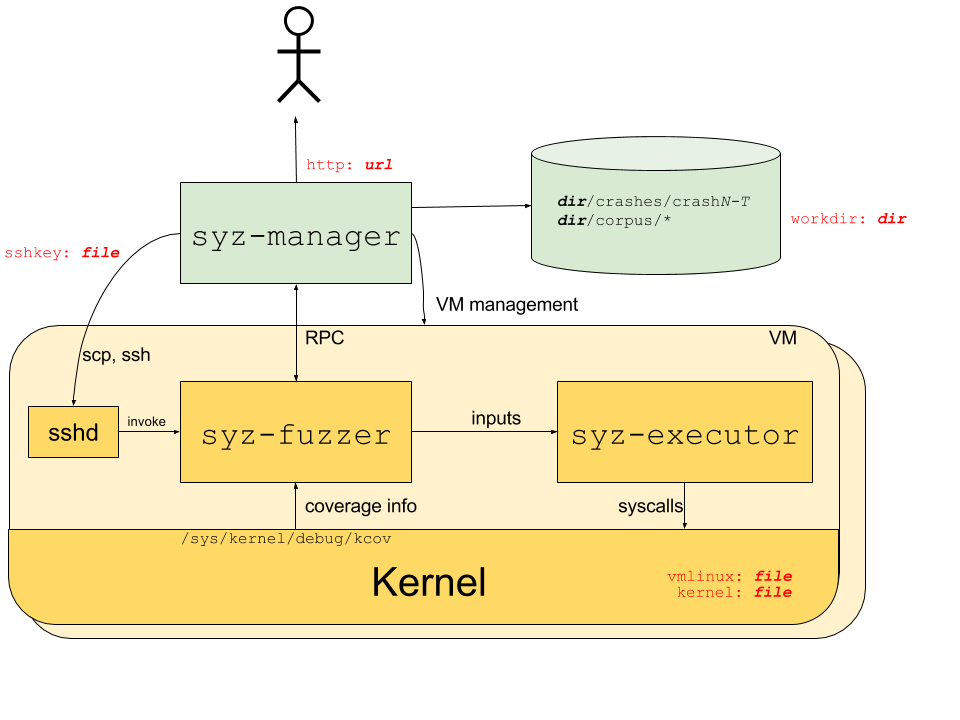
\includegraphics[width=.9\linewidth]{tex/img/syz.png}
    \caption{The diagram of \textit{Syzkaller} fuzzer}
    \label{fig:syz}
\end{figure}

\subsection{Operating systems and platform emulation}
Operating system are designed to run on bare hardware without any emulation or virtualization, with direct access to hardware. For this reason, the kernels are heavily reliant on the provided hardware and don't allow for running a second operating system. To address this issue, engineers started creating emulators which were capable of running foreign code and simulate a particular hardware from the emulated architecture. The first \textit{Intel x86} virtual machines managers allowing system emulation were released by \textit{VMWare} in 1999 as stated in \cite{vms}. This was accelerated by the introduction of the \textit{Vt-x} Intel CPU features. This virtualization extension allowed for hardware acceleration of processor emulation. In detail, it provides isolation between emulated and physical processors, so the virtual machine manager only needs to manage the emulated hardware. This improvement eliminated the need to emulate CPU instruction in the emulator's code, thereby making the virtual machine run almost as fast as the host. Of course, since \textit{Vt-x} is a processor extension, this didn't simplify emulating hardware inside a virtual machine and the virtual machine manager is still required to either fully emulate a virtual component or pass-through the real ones from the host. 

Later, the \textit{QEMU} or the \textit{Quick EMUlator} project was created at \cite{qemurepo}. It allowed for easy emulation of various hardware and processors architectures. As a result, \textit{QEMU} has a sophisticated architecture consisting of several modules and platforms descriptions. Each platform represents an emulated hardware, it can be chosen from a variety of types from a generic Intel x86 to a very specific embedded ARM CPU or even some old architectures like SPARC.

\subsubsection{QEMU emulator architecture}

Emulating operating systems requires simulating the CPU as well as the hardware. To accomplish this, \textit{QEMU} employs various techniques. Firstly, to emulate the CPU, we have the choice between hardware accelerated virtualization and full software emulation. The acceleration uses features built-in to the CPU to provide isolation between virtual machines and the host. The disadvantage is that it only works when the emulated processor is of the same architecture. To simulate an incompatible processor, every instruction needs to be simulated in software. Such translation is similar to, for example, how a \textit{JIT} compiler operates. The module in \text{QEMU} responsible for that is called the \textit{Tiny Code Generator}, or simply the \textit{TCG}. For clarity, all described below components have been put in a diagram available in figure \ref{fig:qemuarch}.

\paragraph{\textit{Tiny Code Generator}}
The \textit{TCG} module, as described in \cite{qemutcg}, can be split into two parts. The former is translating the emulated CPU instructions into a virtual intermediate assembly called \textit{QEMU OPS}. The latter is translating the intermediate code into host architecture. This design allows for robustness as every supported architecture can be emulated on all of them. This also adds the possibility to modify, that is, instrument the running code at runtime. Additionally, this allows for extending the simulated instruction set by adding new encodings or modifying existing instructions.

The \textit{QEMU OPS} virtual architecture implements a \textit{RISC} like processor with simple load, store and arithmetic operations. This is of course sufficient to simulate all  complicated instructions of a \textit{CISC} processor like for ex. Intel x86. Therefore, the designers of \textit{QEMU} implemented a mechanism allowing to just register a callback function to be run when the translated instruction is executed. This is a very powerful mechanism, as the callback has access to both the emulated system and the \textit{QEMU} process running on the host. This allows not only emulating very complicated instructions of a \textit{CISC} processor, but also instruction used to communicate directly with the emulator. Such instructions are called \textit{hyper calls}, since they are used to communicating with the \textit{hypervisor}.

An example of an intermediate assembly is shown in listing \ref{lst:tcgir}. It can be seen that most of the instructions are of arithmetic type that can operate on registers and a couple of special ones to interact with memory or QEMU internals. At the end there are several interesting orders:
\begin{itemize}
    \item \textit{qemu\_st\_i32 r0,tmp0,beul,3} - this is the memory access operation that stores data (from \textit{r0}) on address (\textit{tmp0}), the next 2 arguments specific the access type (endianess, bus width) and memory index which selects kernel and user memory, naturally there exists an equivalent \textit{qemu\_ld\_i32} load instruction,
    \item \textit{call        store\_msr,\$0,tmp0} - this will call the \textit{store\_msr} TCG helper which is a function complied into QEMU, here \textit{\$0} represents the return value and then follows the parameter list,
    \item \textit{set\_label   \$L0} - this instruction is used to assign a label to the current address which can later be used as arguments in branching,
    \item \textit{exit\_tb     \$0x7f5a0caf8043} - this is a special opcode which exists from the translated code to QEMU, here it is most likely the translation unit which will proceed with the preparation of next code block.
\end{itemize}

\begin{minipage}{\linewidth}
\begin{lstlisting}[caption={QEMU TCG intermediate assembly code from \cite{qemutcgir}},label={lst:tcgir}]
0xfff00100:  movi_i32    r1,$0x10000

0xfff00104:  movi_i32    tmp0,$0x409c
             or_i32      r1,r1,tmp0

0xfff00108:  movi_i32    r0,$0x0

0xfff0010c:  movi_i32    tmp1,$0x4
             add_i32     tmp0,r1,tmp1
             qemu_st_i32 r0,tmp0,beul,3

0xfff00110:  movi_i32    nip,$0xfff00114
             mov_i32     tmp0,r0
             call        store_msr,$0,tmp0
             movi_i32    nip,$0xfff00114
             exit_tb     $0x0
             set_label   $L0
             exit_tb     $0x7f5a0caf8043
\end{lstlisting}
\end{minipage}

\paragraph{\textit{Thread structure}}
To run the virtual machine \textit{QEMU} uses different threads to do different tasks, as described in \cite{qemuthreads}. The main thread called the \textit{Mainloop} is responsible for controlling the emulated machine. It exposes an interface for scheduling tasks and controls the main event loop. All tasks requiring the virtual machine to be in a consistent state are executed in the context of the \textit{Mainloop} thread. The reason being that this thread can halt and shutdown other threads when needed. Consequently, scheduled tasks can operate on synchronized state of all virtual CPUs. One of such tasks is, for example, taking or restoring a snapshot. While the virtual machine is saved, all other threads are suspended and resumed after the operation is finished. Furthermore, the \textit{Mainloop} is also responsible for handling the user interface known as \textit{QEMU monitor}. It allows for controlling the virtual machine from command line.

Next, to emulate the hardware and interrupts, \textit{QEMU} uses a separate thread called the \textit{IOThtread}. It's also an event loop, but this time it's processing event from emulated hardware. There might be many of such threads, but for small systems like embedded processors, one is usually enough. suspending this thread is essential to ensure that the virtual hardware can be safely inspected and operated on from outside.

Last, but not least, there are the \textit{vCPU} threads. These are responsible for the described instruction translation and then execution. In the beginning, the emulated assembly code is split into parts called basic blocks. Each block is then translated using the \textit{TCG} module to host machine code. It is stored in an executable memory region. After the translation, \textit{QEMU} starts executing the generated code by simply jumping to it. To speed this process up, \textit{TCG} caches translated blocks as not to recompile same fragments many times over. 

\tikzstyle{qemu} = [rectangle, minimum width=3cm, minimum height=1cm,text centered, draw=black, fill=green!10]
\tikzstyle{thread} = [rectangle, minimum width=3cm, minimum height=1cm,text centered, draw=black, fill=orange!30]
\tikzstyle{module} = [rectangle, text width=2cm, minimum height=1cm,text centered, draw=black, fill=yellow!30]
\tikzstyle{darrow} = [thick,<->,>=stealth]

\begin{figure}[h!]
    \centering

    \begin{tikzpicture}
        \node (qemu) [qemu, text width=10cm, text height=11cm, label=north:QEMU] {};

        \node (main) [thread, yshift=-4cm, text width=8cm, text height=2cm, label=north:Mainloop] {};
        \node (vcpu) [thread, text width=2cm, text height=6cm, yshift=1.5cm, xshift=-2cm, label=north:vCPU] {};
        \node (iothread) [thread, text width=2cm, text height=6cm, yshift=1.5cm, xshift=2cm, label=north:IOThread] {};

        \node (tcg) [module, xshift=-2cm, yshift=3.5cm] { TCG };
        \node (code) [module, below of=tcg, yshift=-1cm] { Emulated code };
        \node (state) [module, below of=code, yshift=-1cm] { Virtual CPU state };
        \node (io) [module, xshift=2cm, yshift=3.5cm] { Emulated hardware };
        \node (ioevent) [module, below of=io, yshift=-1cm] { Event loop for interrupts };
        \node (user) [module, yshift=-4cm, xshift=-2cm] { User interface };
        \node (event) [module, right of=user, xshift=3cm] { Main event loop};

    \end{tikzpicture}
    
    \caption{QEMU architecture diagram}
    \label{fig:qemuarch}
\end{figure}

\subsubsection{Trustzone technology} \label{sec:tz}
Each contemporary \textit{CPU} architecture implements a module responsible for providing security features, which is isolated from the main operating system. This way, application developers can create more secure services. Each service can store secrets inside encrypted secure memory or derive keys for encryption and signature verification. Thanks to this, the compromise of the main operating system might not lead directly to the leakage of sensitive data. In \textit{ARM} CPU, this technology is implemented as a more privileged mode of the CPU. It is named \textit{Trustzone} and defined in \cite{trustzonedoc}.

\begin{figure}
    \centering
    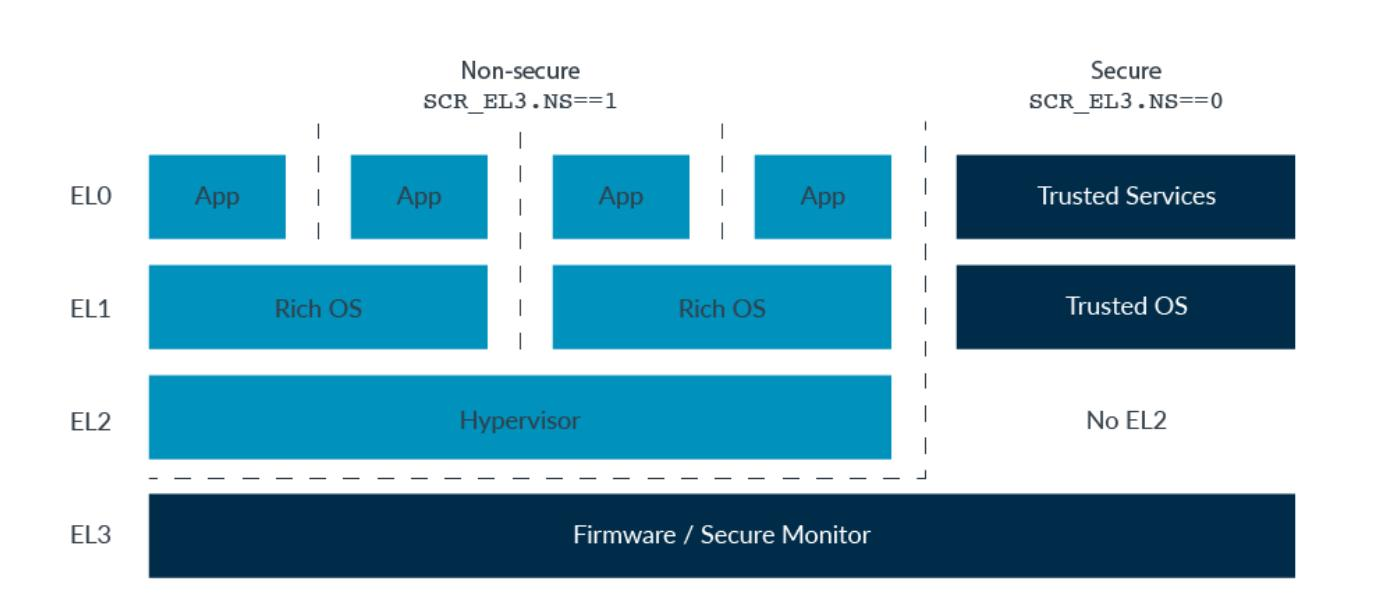
\includegraphics[width=.9\linewidth]{tex/img/trustzone.jpg}
    \caption{Example \textit{Trustzone} implementation in \textit{armv8} architecture}
    \label{fig:tzarmv8}
\end{figure}

The diagram showing the security architecture of \textit{armv8} processor is shown in figure \ref{fig:tzarmv8}. The major difference between this architecture and, for example, the \textit{Intel x86} is the existence of other so-called worlds. There is a non-secure world, where the "normal" operating system, like for example \textit{Android} lives. The latter called the secure world provides space for the special security oriented operating system. On the architectural level, the worlds are implemented by selectively allowing and forbidding access to parts of physical memory based on whether the CPU is running in secure or normal mode. The non-secure world is sometimes called the rich world, as it doesn't implement this many security enhancements as the secure one.

 Apart from different worlds, the CPU employs different privilege modes to separate running code. There exist four different levels:
\begin{enumerate}
    \item \textit{EL0} - the least privilege one, all applications run here
    \item \textit{EL1} - the level on which runs the operating system
    \item \textit{EL2} - hypervisor level, it is used to manage virtual machines running in non-secure mode
    \item \textit{EL3} - the secure monitor mode, it is responsible for providing separation between worlds and communication with hardware
\end{enumerate}

\subsubsection{OPTEE OS}
\textit{OPTEE OS} is an open source, security oriented operating system designed specially for \textit{Trustzone} technology. It consists of a core written in \textit{C} and applications called \textit{Trusted Application} or in short “TA's”. Each such application can expose an interface to either another \textit{TA} or as a service in the non-secure world. The architecture diagram can be seen in figure \ref{fig:optee}. As we can see from the diagram, \textit{OPTEE OS} kernel and application live solely in the secure world and talk to the non-secure through a communication channel provided by the \textit{CPU}. The non-secure world then utilizes a device driver to call secure services. The tasks of such operating system are wide and range from verifying code signatures through key derivation to storing data securely in encrypted memory. An example of how this technology can be used is provided in \cite{opteeusage}. There, the researchers describe developing security mechanism useful in \textit{IoT} or \textit{Internet of Things} devices. The article focuses on different aspects of security:
\begin{enumerate}
    \item Confidentiality – making sure that the stored information is available only to authorized appliances, 
    \item Integrity – attesting data and software to detect malicious tampering,
    \item Authorization – to perform security check on the system,
    \item Availability – ensure that the security module is always available,
    \item Privacy – the need to keep all information confidential.
\end{enumerate}

\paragraph{\textit{OPTEE OS} architecture}
As a result of \textit{OPTEE OS} being a secure-oriented OS, its application interface provides a lot of cryptography related functions. It implements many symmetric and asymmetric ciphers along with hash functions. Though the system doesn't implement a casual file system, it has a secure encrypted storage which can be accessed from the non-secure world. This allows for creating an application with a special secure part running in \textit{Trustzone} which handles all sensitive operations. Of course, the security of the entire system relies on the security of the secure driver. If there is any vulnerability inside, it may compromise the secure service. Naturally, this is not easy as one must find first a vulnerability in the non-secure application to even reach the secure part, so the isolation add a level of complexity to a potential attack. As an open source project, \textit{OPTEE OS} can be deployed on a couple of hardware platforms, such as the \textit{Raspberry Pi} family and other board having an \textit{ARM} CPU with \textit{Trustzone} support. Thankfully, it can also be emulated in \textit{QEMU} using the default \textit{ARM} virtual machine board definition. This makes testing and development easy as it's not required to acquire some special proprietary hardware.

\begin{figure}[h!]
    \centering
    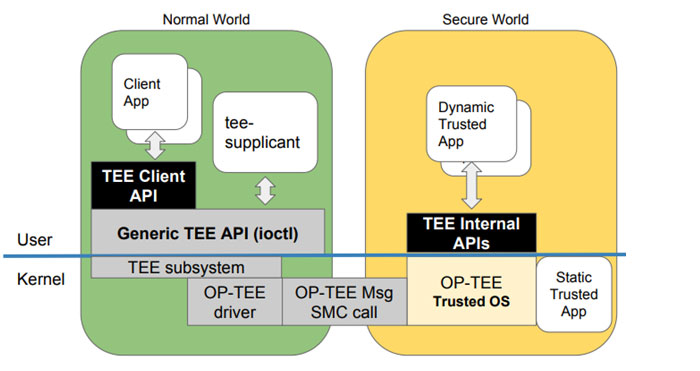
\includegraphics[width=.8\linewidth]{tex/img/op-tee-software-architecture.jpg}
    \caption{\textit{OPTEE OS} architecture diagram from \cite{opteeblog}}
    \label{fig:optee}
\end{figure}


\subsection{Rust}

\textit{Rust} programming language is a recently created, primarily targeted for system programmers. The design of this language is available in so-called \textit{Rust book} in \cite{rustbook}, which is a comprehensive description of features and design choices.  It's advertised as a \textit{C/C++} successor in the fields of operating systems, driver and operating system services development. Therefore, \textit{Rust} supports many architectures and operating systems. Additionally, it can be compiled without any external dependencies, or in so-called bare metal environment, to be used as operating system. As every modern programming language, Rust comes with its own package manager, which allows for easy dependency management. Each project from the point of view of the package manager is called a crate. Such entity consist of a crate manifest and source files. The Rust designers have also divided crates into two types, there can be library crates which can only expose functionalities and executable crates which are then compiled to a binary.

\paragraph{Advantages of Rust}
\textit{Rust} introduces new security mechanism which are absent in the family of languages derived from \textit{C}. Primarily, \textit{Rust} focuses on memory and thread safety like stated in \cite{rustmemorysafety}. First, \textit{Rust} abandons the use of pointers and allows only references. This enhancement is motivated by a lot of bugs found in non \textit{Rust} software, being memory corruption. Along to disallowing the use of pointers inside the so-called safe code, Rust introduces lifetime checking of references. This module was named the borrow checker, its task is to ensure that all entities live in memory as long as they are used. This eliminates other memory bugs such as the popular “use-after-free” where an object is destroyed, yet there still exists a reference to the freed memory and other parts of the program are still executing as if the object still existed. An example of such code can be seen in listing \ref{badcpp} written in \textit{C++}. In this code, the function creates on the stack a local variable named \textit{var} and assigns a value of 0. Then the code takes a reference to \textit{var} and returns it from the function. This, results in accessing unallocated memory, as the variable is allocated in the beginning of the function and freed just before returning. In comparison, listing \ref{badrust} shows the equivalent code in \textit{Rust}. Here, just like in the \textit{C++} example, the code allocates on the stack a 32-bit signed variable and assigns a value of 0. Then it proceeds with returning a reference to it. For clarity, in \textit{Rust} the value of the last expression in a function is treated as the return value. Hence, there is no need to explicitly use the \textit{return} keyword, although \textit{Rust} support it. As expected, the \textit{C++} example compiled without issue, only emitting a warning that can be silenced, whereas Rust terminates the compilation with a message stating that the return value of the function lives not long enough. Additionally, Rust controls how references to variables are created. There are two major rules:
\begin{enumerate}
    \item an object can have immutable references if and only if it doesn't have any mutable reference,
    \item an object cannot have multiple mutable references.
\end{enumerate}
These restrictions ensure that objects doesn't suddenly change or became deleted while other objects still use them.

Apart from that, Rust's assignment operation moves the argument instead of copying it, as it is the case in languages like C++. This allows for writing efficient code, as each copy operating needs to be explicitly allowed. Besides that, the language provides a mechanism to securely pass entities between threads. Basically, Rust bans the usage of an object in a multithreaded environment if it doesn't implement the proper synchronization mechanisms. This eliminates race conditions where threads race for access to a shared resource and different order of accesses leads to different execution results. Unfortunately, this doesn't solve the problem of two threads locking up on a shared pair of resources, stalling the execution forever. Therefore, the deadlock problem is still persistent and needs to be avoided. 

\begin{minipage}{.4\textwidth}
    \begin{lstlisting}[language=c++,caption={Example of a memory corruption bug in C++},captionpos=b,label={badcpp}]
int& function() {
    int var = 0;
    return &var;
}
    \end{lstlisting} 
\end{minipage}
\hfill\vline\hfill
\begin{minipage}{.4\textwidth}
    \begin{lstlisting}[language=rust,caption={Replicating a memory corruption bug in Rust},captionpos=b,label={badrust}]
fn function() -> &i32 {
    let var = 0i32;
    &var
} 
    \end{lstlisting}
\end{minipage}

Rust designers have also abandoned the use of inheritance as a polymorphism mechanism, they instead introduced traits. Each trait defines an interface which can be implemented by a struct, which then allows the object to be referred to as a reference to the trait it implements. This effectively replaces the inheritance, without the potential complications that can arise like, for example, diamond inheritance. For clarity, this class derivation scheme happens when some base class exists in multiple instances in the inheritance tree. Normally, this situation is impossible in languages like \textit{C\#} or \textit{Java} where a class can only inherit from a single base class. As a result, all inheritance schemas are trees, usually starting from a single base class. However, \textit{C++} language allows for multi base inheritance, which can lead to complicated structures in the derivation graph.

%The simplest diamond inheritance case is shown in figure \ref{fig:dinher}. 

%\begin{figure}[h!]
%    \centering
%
%    \begin{tikzpicture}
%        \node (A) [module] { A };
%        \node (B) [module, below of=A, xshift=2cm, yshift=-1cm] { B };
%        \node (C) [module, below of=A, xshift=-2cm, yshift=-1cm] { C };
%        \node (D) [module, below of=A, yshift=-3cm] { D };
%
%        \draw [arrow] (A) -| (B);
%        \draw [arrow] (A) -| (C);
%        \draw [arrow] (B) |- (D);
%        \draw [arrow] (C) |- (D);
%    \end{tikzpicture}
%    
%    \caption{Diamond inheritance graph example}
%    \label{fig:dinher}
%\end{figure}

The only limitation that is imposed on what trait can be implemented for which type is that one may not implement a foreign trait for a foreign type. The word foreign means here an entity outside the crate that's providing the trait's implementation. This is done, to not allow for extending external types with new implementation. We might imagine that if it was the case, this could result in many incompatible implementations which would break the project.

\paragraph{Unsafe code}
Sadly, while creating an operating system, this security rules cannot be upheld for each code line. Just like stated in \cite{rusthowunsafe}, there are situations where the security checks need to be disabled for a part of code. Almost all such cases involve talking to computer hardware. Currently, the hardware still has an ugly interface requiring the use of pointers, buffers, and flags or status codes. This, of course, violates the \textit{Rust}'s security rules. Therefore, while developing the code which directly accesses the hardware, some restrictions must be lifted. This is done using the \textit{unsafe} keyword, which defines a code block or a function where \textit{Rust} allows pointers and doesn't check whether the memory is properly managed. Inside those blocks, tasks like memory management and thread synchronization once again rely fully on the programmer. As a result, this might introduce bugs and security vulnerabilities like shown in \cite{rustunsafeissues}, which the designers of Rust want to eliminate. Therefore, the usage of unsafe code should be limited only to required cases and thoroughly reviewed. An example of such use case is shown in listing \ref{unsafe_rust}. As it can be seen, the code defines a variable holding an address to a memory mapped register. This is a perfectly safe operation as it's just assigning an integer value. However, the next operation violates the security rules. In the next 3 lines, the address will be cast from an integer to an unsigned \textit{int} pointer and then dereferenced. From these two actions, only the dereferencing is unsafe and needs to be enclosed with an \textit{unsafe} block. The reason for it being unsafe is that the \textit{Rust} compiler cannot assert whether this pointer is valid, as it was just converted from an arbitrary numerical value. 

\begin{minipage}{.9\textwidth}
    \begin{lstlisting}[language=rust,caption={Unsafe code exmaple},captionpos=b,label={unsafe_rust}]
fn read_register() -> u32 {
    let address = 0x20000020 as u32;
    unsafe {
        *(address as *const u32)
    }
}        
    \end{lstlisting}    
\end{minipage}

\subsubsection{\texttt{proc macro} mechanism}
Rust programming language lack the usual meta programming tools:
\begin{itemize}
    \item text preprocessor, like that in "C"
    \item templates engine like that in "C++", although Rust does have generics, they aren't as powerful as those in C++.
\end{itemize}
As a result, Rust language designers created another, even more capable mechanism named macros. Instead of, extending what generics can do as it happened in case of \textit{C++}, the designers came up with a tool which processes tokens from the source code. It is far superior to a simple text processor, as is can distinguish entities based on \textit{Rust}'s syntax and not only raw text. On the same time, it is way easier to employ than \textit{C++} template system as these macros take as input a stream of tokens which can be matched into different patterns and output another stream of tokens without the need to spend hours trying to code everything functionally using \textit{C++} templates. 

Sometimes, a simple macro processing tokens is not enough. To cover all other use cases, the language creators designed the so-called procedural macros. These are essentially functions which process tokens and return tokens. They are compiled first during the build process and are invoked by the compiler to generate code which will be compiled along with the rest of the source code. What makes such macros really powerful is lack of limits of what such macro can do. It can even make an internet connection to download some code and add it to the compiled binary. This allows for a huge variety of things that can be done during compile time. 
However, what's most interesting is the ability to extend the Rust compiler with procedural macros able to transpile some language into rust. This allows programmers to develop custom languages and seamlessly incorporating them into Rust.


To shed some light on \textit{proc} macros, a simple example can be seen in listing \ref{lst:procmacrodef}. It starts with a special attribute \textit{\#[proc\_macro]} which tells the \textit{Rust} compiler that it should treat the function below as a \textit{proc} macro. Like every such macro, the \textit{implement\_magic} takes a \textit{TokenStream} object as argument and returns a \textit{TokenStream}. In detail, the \textit{TokenStream} struct represents the \textit{Rust} compiler's token stream. The function then takes a text literal with \textit{Rust} code inside, which defines a function named \textit{magic}, and converts it to \textit{TokenStream} by calling the \textit{parse()} member function. Finally, these tokens are returned, as this is the last expression in the function's body. The \textit{proc} macros, like the described one, can be later used in another crate, as shown in listing \ref{lst:procmacrousage}. There, the \textit{main} function calls the \textit{magic} function, which doesn't appear to be defined anywhere. However, above the definition of \textit{main} the \textit{implement\_magic} macro is invoked. After the macro finished executing, the call place is replaced with the tokens from its return value. Basically, it provides the definition of \textit{magic} function in this case.

\begin{minipage}{\linewidth}
\begin{lstlisting}[language=rust,caption={Exmaple of a \textit{proc} macro definition},label={lst:procmacrodef}]
#[proc_macro]
pub fn implement_magic(tokens: TokenStream) -> TokenStream {
    "fn magic(x: u32) -> u32 { 0xAA * x + 1 }".parse().unwrap()
}
\end{lstlisting}
\end{minipage}

\begin{minipage}{\linewidth}
\begin{lstlisting}[language=rust,caption={Exmaple usage of a \textit{proc} macro},label={lst:procmacrousage}]
implement_magic!();

fn main() {
    println!("x = {}", magic(1));
}
\end{lstlisting}
\end{minipage}

\subsubsection{Creating compiler using \textit{syn} and \textit{quote} crates}
As discussed above, procedural macro allow for an easy creation of what is essentially a compiler inside Rust compiler. To aid in this task, Rust provides the \textit{syn} and \textit{quote} create, which can be used for parsing input and generating output. The \textit{syn} crate contains everything required to parse Rust code, along with interfaces to create custom entities and tokens. This crate provides the \textit{Parse} trait which, when implemented, allows the Rust compiler to treat it as if it was a part of the language. After the successful parsing, we are left with the syntax tree. The next step is to proceed to the code generation step. Here the language helps by providing the \textit{quote} macro. It is a helper which allows constructing a token stream from rust code. A very simple use of those crates can be a macro adding tracing to the program. In listing \ref{proc_macro} we can see a macro that rewrites the argument by adding a line that prints the function's name. It starts with parsing the input as \textit{ItemFn} which represents a function in the \textit{Rust}'s syntax tree. This struct holds all relevant information about a function:
\begin{enumerate}
    \item \textit{attrs} - this array holds all function attributes, these can be other macros or compiler defined special statements,
    \item \textit{vis} - this is the visibility attribute which can take 3 value: public, private or inherited,
    \item \textit{sig} - the function's signature, it holds the label, generic parameters and function's arguments with their definition along with the return value type,
    \item \textit{block} - this array holds list of statements from the function's body.
\end{enumerate}
All these fields are then in line 4 extracted from the \textit{ItemFn} struct and in the following 2 lines just for convenience two references to the name and list of statements are taken. In the end, the \textit{add\_trace} function generates code using the \textit{quote} macro. This macro is provided with specially augmented \textit{Rust} code. It can be seen that some identifiers are preceded with \textit{\#} or \textit{\#(\# )\*}, these are part of the special language \textit{quote} macro employs. These two attributes mean the following:
\begin{itemize}
    \item a single \textit{\#} before a variable's name will replace its occurrence with its tokenized value, for example if a variable holds a text literal it will be tokenized as this literal enclosed in double quotes,
    \item the \textit{\#(\#variable)\*} notation assumes that the variable is an array and will repeat what's inside the parenthesis for each element of the array.
\end{itemize}
All these actions are taken to rewrite the function and add a \textit{println} statement at the beginning of this function's body. It can be seen that the attributes, the visibility is rewritten without modification. Then inside the body a \textit{println} statement is added which prints the function's name. Next follows the expanse of the statements list. Since the additional line is added at the beginning, this doesn't have any impact on the return value.

\begin{minipage}{.9\textwidth}
    \begin{lstlisting}[language=rust,caption={A procedural macro exmaple},captionpos=b,label={proc_macro}]
#[proc_macro]
pub fn add_trace(item: TokenStream) -> TokenStream {
    let input: ItemFn = parse_macro_input!(item);
    let ItemFn { attrs, vis, sig, block } = input;
    let name = &sig.ident;
    let stmts = &block.stmts;
    quote! {
        #(#attrs)* #vis #sig {
            println!("TRACE {}", #name);
            #(#stmts)*
        }
    }
}
    \end{lstlisting}
\end{minipage}

\paragraph{SSA compiler} \label{ssadec}
Designing a compiler is a very challenging and technically complicated task. As a result, researchers studied this field and came up with various approaches designed to simplify all the required compilation steps. One of such designs is the \textit{Static Single Assignment} or \textit{SSO} in short. As described in \cite{ssabook}, this method imposes a restriction on how variables can be used. In a nutshell, whenever an assignment operation is taking place, a new variable shall be allocated. This simplifies the optimization algorithms, as now each value of a variable can be symbolically expressed as a tree of operations. It helps the compiler deduce properties of expressions. An example showing the differences between a code written without the rules of SSA can be seen in listing \ref{code_1} and that in SSA form in \ref{code_2}. It can be seen that in the non SSA form the \textit{x} variable is assigned twice, therefore its value may change between lines 2 and 4. As a result, there is no single and simple symbolic expression for the value assigned to label \textit{x}. On the other hand, the SSA compatible form example does assign a new label to the \textit{x} variable in line 3. Therefore, it's easier to see how values depend on each other. Additionally, it's beneficial in the context of creating a compiler macro like described above. Since rust forbids taking multiple mutable references to a variable or any immutable whenever a mutable reference exists, keeping everything constant and just reallocating values makes the design already complaint with the language rules. For this reason, this representation will be used in the code generator part of the compiler designed in this thesis.

\begin{minipage}{.4\textwidth}
    \begin{lstlisting}[language=C,caption={Code exmaple containing assigments},captionpos=b,label={code_1}]
<@$x$@> = 1
<@$y$@> = <@$x$@> + 2
<@$x$@> = 4
<@$z$@> = <@$x$@> + 2
    \end{lstlisting}
\end{minipage}
\hfill\vline\hfill
\begin{minipage}{.4\textwidth}
    \begin{lstlisting}[language=C,caption={Code exmaple in SSO notation},captionpos=b,label={code_2}]
<@$x_0$@> = 1
<@$y_0$@> = <@$x_0$@> + 2
<@$x_1$@> = 4
<@$z_0$@> = <@$x_1$@> + 2
    \end{lstlisting}    
\end{minipage}
\cleardoublepage
\section{What do we want to achieve and how?} \label{chap:why}
In order to succeed with the task of \textit{fuzzing} custom operating systems, I needed to find a quick way of running a test, recording and analyzing the results. The analysis part is usually performed by genetic algorithms embedded in \textit{fuzzers}. Therefore, the designed solution should easily integrate with a well known \textit{fuzzer}. In my case, being inspired by the \textit{Triforce AFL} project from \cite{triforceafl}, I have chosen the \textit{AFLplusplus} \textit{fuzzer}. The next element in the puzzle is the emulator. There are a lot of widely available solutions, but most of them aren't open source, which makes modification a real hassle. This narrows the choice to \textit{QEMU} and \textit{Xen}. Due to my experience with, \textit{QEMU} I've chosen this over \textit{Xen}. The target is a service running in the secure world in so-called \textit{Trustzone}. It runs under \textit{OPTEE OS} operating system and performs a couple of security operations. Since the application runs in \textit{Trustzone}, QEMU needs to exactly emulate a version of ARM which supports it. The host architecture is the \textit{Intel x86} as the tests are executed on an off-the-shelf laptop computer. 

The \textit{Trustzone} technology was designed to provide services for applications running in the normal mode. Therefore, part of the setup is also be present in the \textit{Linux} operating system in the normal world. Its role is to set everything up and begin \textit{fuzzing} by loading the special trusted application and invoking the function which starts \textit{fuzzing} in the secure world. On the other hand, the secure world part is responsible for communication with the \textit{AFL} \textit{fuzzer} through \textit{QEMU}. Furthermore, this is the part that calls the secure services. In an everyday situation, those services would be exposed to the normal world, but since this is just a demonstration setup, the fuzzer was integrated directly. On the other hand, calling services indirectly from normal world would most likely add some needless latency. Besides that, the secure part also performs the test case interpretation and the final function calls. 

\subsection{Requirements for the emulator}
This part of the setup has the most impact on \textit{fuzzing} speed, as executing a test case takes much more time when compared to evaluating the results in \textit{AFL}. This is primarily caused by the fact that the target is an entire operating system. Additionally, when the emulated OS has different CPU architecture than the host OS, the instructions need to be emulated in software, which usually brings a lot of overhead. Therefore, all modifications to the emulator need to be as efficient as possible, not to waste more CPU time than required. The main tasks of the modified emulator are to communicate with the \textit{fuzzer} and bring the operating system back up after each crash. The communication can be established by adding special virtual CPU instructions. As for storing the virtual machine state, many options and restoring policies will be evaluated to check which performs best.

\subsection{Requirements for the test case interpretation}
This thesis is about \textit{fuzzing} services provided by a secure operating system which are written in \textit{Rust}. Therefore, the \textit{fuzzer} needs to support a subset of \textit{Rust} language, which is enough to perform function calls and handle objects. The application provides the description of the target functions and classes to generate appropriate deserialization methods. It is provided via a simple declarative language designed specially to allow for specifying how to call functions using a simple set of primitives that can be directly created from the test case. Then, the \textit{fuzzer} implements a compiler that transpiles the target description into \textit{Rust} code. The generated code implements the actual \textit{fuzzing} routines, thus this solution can be classified as a \textit{fuzzer} generator. Finally, the compiler generates macros allowing for generating test cases from function calls, a process that acts backwards to the \textit{fuzzing}. This will be helpful in creating a corpus for \textit{fuzzer} using existing unit test suits. 

\subsection{Fuzzing architecture}
For clarity, figure \ref{fig:fuzzoverview} shows all the software components with data flow paths. To distinguish between components which were created in this thesis and the open source ones, different colors were used:
\begin{itemize}
    \item \colorbox{green!30}{light green} - marks an open source project which was only slightly modified or adapted,
    \item \colorbox{orange!30}{orange} - marks components which were fully created by me,
    \item \colorbox{yellow!30}{yellow} - marks components whose modification were required,
    \item \colorbox{green!60}{green} - marks an unmodified open source component.
\end{itemize}
In detail, the \textit{fuzzing} setup consists of three main components:
\begin{enumerate}
    \item The \textit{AFL++} \textit{fuzzer} described in section \ref{sec:afl}.
    \item The \textit{AFL to QEMU interface translator} whose role is to connect the \textit{fuzzer} to QEMU, its implementation is provided in section \ref{sec:translator}.
    \item The \textit{Fuzzer integration} described in \ref{sec:savevm} implements primarily the saving and restoring of the virtual machine state mechanism.
    \item The \textit{Tiny Code Generator} is the instruction translator in \textit{QEMU} which provides a communication channel with the \textit{Test case decoder} as shown in \ref{sec:tcg}.
    \item The \textit{OPTEE OS} is the special operating system running in \textit{Trustzone} as described in \ref{sec:tz}.
    \item The \textit{Buildroot} which runs in the normal world and simulates the user of secure world's services.
    \item The \textit{Initializer} is a simple application running under \textit{Buildroot} which is responsible for loading the trusted application package containing the test case decoder and secure services.
    \item The \textit{Test case decoder} decodes the test case's bytes into function calls, it is described in section \ref{sec:testcase}.
    \item The \textit{Secure services} is an application written in \textit{Rust} that utilizes \textit{OPTEE OS} kernel's secure APIs, it is the target of \textit{fuzzing}.
\end{enumerate}

\tikzstyle{opensource} = [rectangle, minimum width=3cm, minimum height=1cm,text centered, draw=black, fill=green!30]
\tikzstyle{custom} = [rectangle, minimum width=3cm, minimum height=1cm,text centered, draw=black, fill=orange!30]
\tikzstyle{opensourcemod} = [rectangle, minimum width=3cm, minimum height=1cm,text centered, draw=black, fill=green!60]
\tikzstyle{custommod} = [rectangle, minimum width=3cm, minimum height=1cm,text centered, draw=black, fill=orange!60]
\tikzstyle{modifiedmod} = [rectangle, minimum width=3cm, minimum height=1cm,text centered, draw=black, fill=yellow!30]
\tikzstyle{host} = [rectangle, minimum width=3cm, minimum height=1cm,text centered, draw=black, fill=brown!30]

\tikzstyle{arrow} = [thick,->,>=stealth]
\tikzstyle{darrow} = [thick,<->,>=stealth]

\pgfdeclarelayer{background0}
\pgfdeclarelayer{background1}
\pgfdeclarelayer{background2}
\pgfsetlayers{background0, background1, background2, main}

\begin{figure}[h!]
    \centering

    \begin{tikzpicture}
        \node (kernel) [opensourcemod, text width=3cm] { OPTEE kernel };
        \node (target) [custommod, below of=kernel, text width=2cm, yshift=-0.5cm] { Secure services };
        \node (fuzzer) [custommod, text width=2cm, below of=target, yshift=-0.5cm] { Test case decoder };

        
        \begin{pgfonlayer}{background1}
            \node (optee) [opensource, fit={(fuzzer) (target) (kernel)}, text width=4cm, text height=5cm, label={OPTEE OS}] {};
        \end{pgfonlayer}
        
        \node (kernel2) [opensourcemod, text width=3cm, right of=kernel, xshift=4cm] { Linux kernel };
        \node (fuzz2) [custommod, below of=kernel2, yshift=-0.5cm] { Initializer };

        \begin{pgfonlayer}{background1}
            \node (buildroot) [opensource, fit={(kernel2) (fuzz2)}, text width=4cm, text height=3.5cm, label={Buildroot}] {};
        \end{pgfonlayer}

        \node (fuzzerint) [custommod, below of=fuzzer, yshift=-1.5cm, xshift=0cm] { Fuzzer integration };
        \node (tcg) [modifiedmod, below of=fuzz2, yshift=-3cm] { \textit{Tiny Code Generator }};

        \begin{pgfonlayer}{background0}
            \node (qemu) [opensource, fit={(optee) (fuzzerint) (tcg)}, text width=10cm, text height=8.5cm,label={QEMU}, xshift=0cm] {};
        \end{pgfonlayer}

        \node (gen) [opensourcemod, left of=kernel, xshift=-4.5cm] { Genetic Algorithm };
        
        \begin{pgfonlayer}{background1}
            \node (afl) [opensource, fit={(gen)}, text height=2cm, text width=4cm, label={AFL++ fuzzer}] {};
        \end{pgfonlayer}
        
        \node (srv) [custommod, below of=afl, yshift=-2cm, text width=3cm] { AFL to QEMU interface translator };

        \node (host) [host, below of=qemu, text width=14.5cm, yshift=-4.5cm, xshift=-2cm] { Intel x86 host computer };

        \draw [darrow] (afl) -- (srv);
        \draw [darrow] (srv) |- (fuzzerint);
        \draw [darrow] (fuzzerint) -- (fuzzer);
        \draw [darrow] (fuzzer) -- (target);
        \draw [darrow] (target) --++ (0cm, +1cm);
        
    \end{tikzpicture}
    
    \caption{Fuzzing setup overview.}
    \label{fig:fuzzoverview}
\end{figure}


\cleardoublepage
\section{Modifying QEMU} \label{chap:qemu}

To enable efficient fuzzing in \textit{QEMU}, a couple of design choices must be made. First, a fast communication method between the fuzzer running beside QEMU and the test case executor inside needs to be established. This is required for various reasons, varying from passing simple messages saying that the target is ready to fetch test cases. After the communication channel is established, a compatibility layer must be implemented to integrate \textit{QEMU} with the fuzzer. For example, fuzzers like \textit{AFL} communicate via special file descriptors, shared memory regions, and signals. These file descriptors are both ends of a Linux unnamed pipe created by \textit{AFL} before launching the target. The numbers of those file descriptors are defined in \textit{AFL++} source code as constants. They are respectively 199 for communication to QEMU and 198 in the opposite direction. These are vital to the proper initialization, as it will be discussed later. The shared memory region is used to pass gathered coverage information throughout the test case execution. The main purpose of signals used by \textit{AFL} is just to kill the target if it runs too long. Since a fuzzer cannot know when a test case execution should stop, a firm timer is set. Naturally, figuring out when a test execution will end is equivalent to trying to solve the famous stop problem brought up by Alan Turing. Lastly, after each test case is executed, the target operating system might need to restore itself. It can be as simple as just rebooting it, or some more sophisticated method based on taking a snapshot of the virtual machine state before test case execution and restoring it after.

\paragraph{Chapter content}
This chapter begins with a description of the necessary modifications that need to be applied to the \textit{Tiny Code Generator} module. As previously discussed this enables the communication between the \textit{Fuzzer integration} module and the \textit{Test Case Decoder} running in the emulated environment. Next, it described the \textit{Fuzzer integration} module which implements the additional features required for system fuzzing. One of the most important functionalities added by it is the ability to save and restore the state of the virtual machine. Finally, the implementation of the \textit{AFL to QEMU interface translator} is provided. This is essential to connect the open source \textit{AFL++} fuzzer to \textit{QEMU}.

\subsection{Communicating with the target Operating system}
There are many possible ways of establishing a fast communication channel between \textit{QEMU} and the target operating system. First, the thought might be to add a special device that the target operating system will access when needed. \textit{QEMU} allows to easy creation of any number of virtual devices, from simple memory-mapped devices to sophisticated PCI ones. Unfortunately, this solution has some drawbacks, the main one being that we are using the target operating system to send the information that it has failed. A better way of accomplishing that task would be to use some special assembly instructions. Of course, no such instruction exists in the official instruction sets of real CPUs. The closest to such instruction would be the virtual machine control ones. For example, in Intel x86 architecture, a virtual machine is started using the \textit{vmenter} instruction and exists when the virtual machine executes the \textit{vmexit}. When the exit event happens, the control is passed to the virtual machines' manager, which is the \textit{Kernel Virtual Machine} module inside the Linux kernel. This module is then controlled directly by \textit{QEMU}. Sadly, running this instruction usually requires executing in CPU's kernel mode, as user mode applications can't use those instructions for security reasons. However, since \textit{QEMU} is employed, there aren't any obstacles preventing the addition of a new instruction that would perform the communication and will not have the access control the real hypervisor calls have. In the end, I have chosen to use custom \textit{hypercalls} by modifying the \textit{Tiny Code Generator} module which is responsible for emulating the virtual processor's instructions.

\subsubsection{Modyfing the \textit{Tiny Code Generator}} \label{sec:tcg}
\paragraph{Choosing the special instruction to call QEMU}
In the case of emulating ARM architecture on an Intel x86 host, the instructions are translated by the \textit{TCG} module in \textit{QEMU}. It is therefore required to modify this transpiler, to add a previously unknown instruction and its handler. First, the encoding for the newly added opcode must be found. On \textit{ARM} CPUs instructions have fixed size and the entire space is already completely allocated. Thankfully, there exists the so-called undefined instruction, which by definition guarantees to be undefined. Contrary to its name, it is utilized by various mechanisms, mostly to report errors to the operating system. When such instruction is executed, the operating system delivers a signal to the running application, which in most cases results in the termination of the process. What is interesting in that instruction, is the fact that it can take an immediate argument. The definition of this instruction can be seen in table \ref{tab:armudf}. It shows that there are 2 variants of this instruction, which allow for either 16 or 8 bit immediate parameters. As a result, choosing the encoding comes down to selecting an immediate argument that is not used by anything else inside the operating system. 

\begin{table}[h!]
    \centering
    \begin{tabular}{c|c|c}
        Opcode & Parameters & Instruction set \\
        fx\textsubscript{4}x\textsubscript{2}x\textsubscript{3}fx\textsubscript{1}e7 & 16 bit immediate - x\textsubscript{4}x\textsubscript{3}x\textsubscript{2}x\textsubscript{1} & 32 Bit instruction set \\

        x\textsubscript{1}x\textsubscript{2}de & 8 bit immediate - x\textsubscript{1}x\textsubscript{2} & 16 bit condensed so-called \textit{Thumb} mode \\
    \end{tabular}
    \caption{Definition of the UDF instruction from the Arm manual.}
    \label{tab:armudf}
\end{table}

\paragraph{Adding the instruction to the TCG}
The \textit{TCG} uses bit patterns to assign instruction's mnemonics to encodings. Then after decoding the mnemonic, the TCG parses the arguments based on the instruction type and then calls the proper function that is required to encode it using the QEMU intermediate code, so-called \textit{QEMU OPS}. Naturally, not all instructions are so simple that they are easily describable by a simple RISC-like instruction set. Therefore, the TCG module allows registering a function that has access to the entire emulated CPU state and will be called when the instruction should be executed. Such functions run inside the virtual CPU thread inside QEMU and are not restricted in what they can access as long as proper locks synchronizing QEMU structures are set. As a result, the easiest way to create a communication channel was to add a special instruction with arguments placed in the specially selected registers. Then a callback in QEMU would read those registers and perform the necessary action.

\subsection{Saving and restoring the state of the virtual machine} \label{sec:savevm}
The ability to quickly save and restore the state of the target operating system can be a very useful tool in a couple of situations. First, while executing test cases the global state of the kernel might change, which can result in poorer reproducibility of found bugs. On the other hand, any type of taking and restoring a snapshot will introduce significant delays to the system. It is therefore essential to balance the need to have good reproducibility and fuzzing speed. In detail, the amount of added delay depends solely on the method of taking snapshots chosen. For example, Tamas Lengyel in \cite{xenfuzz} showed a Linux operating system fuzzer based on \textit{Xen} hypervisor. In this solution, he used the built-in save and restore feature. Similarly, the QEMU emulator also provides a native virtual machine serialization mechanism, which will be discussed shortly.

\paragraph{Forking QEMU}
Authors of \cite{triforceafl} tried a different approach to this problem. Since QEMU is just a process running under the Linux operating system, it can be forked or cloned. This is already done and well-supported for emulating single processes inside QEMU. Sadly, this is not the case for full system emulation. The issue with the QEMU system lies in the number of threads it utilizes. Since the QEMU user is just emulating a single user thread, it also utilizes a single thread on the host machine. On the other hand, as already mentioned, the system version of QEMU uses at least 3 threads. This poses a significant obstacle, as forking a multithreaded process on a POSIX system is not supported. What will happen in such a situation is just cloning the thread that is called \textit{fork}. As a result, this is quite tricky to get working, as suddenly creating another \textit{vCPU} thread will certainly crash QEMU.

That is why the researchers designed a sophisticated procedure aimed at making this approach work. To ease out the process, it was divided into two parts. The first seen in figure \ref{fig:preforkqemu} contains all actions up to the point of the fork loop. It starts with the termination of the existing \textit{vCPU} threads, they will be restarted later in the forked thread. When this is completed, the \textit{vCPU} thread schedules a task to be executed in the context of the \textit{IO Thread}. This task is responsible for constantly spawning new \textit{IO Thread} instances by forking itself every time a test case is about to be executed. Thanks to this, each test receives the same copy of the virtual machine. The next part of this process, shown in figure \ref{fig:postfork} displays all action happening in the forked thread. The freshly cloned thread creates the new \textit{vCPU} threads using the copied virtual CPU states and then returns to its normal \textit{IO} event loop. Though this process seems rather straightforward, it is not guaranteed to work reliably in all versions of QEMU. I had severe difficulty in implementing this design to test its effectiveness. Most of the time the QEMU was crashing irregularly and I wasn't able to stabilize it. Therefore, this approach was abandoned, and other ways were explored.

\begin{figure}[h!]
    \centering

    \begin{sequencediagram}
        \newinst[2]{armcpu}{ARM CPU}
        \newthreadShift{vcpu}{vCPU}{2cm}
        \newthreadShift{iothread}{IO Thread}{2cm}

        \mess{vcpu}{Schedule fork loop}{iothread}

        \begin{call}{vcpu}{Stop CPU thread}{armcpu}{}
        \end{call}

        \begin{callself}{vcpu}{wait for io event}{}
        \end{callself}

        \begin{sdblock}{Forkserver}{}
            \begin{callself}{iothread}{endless fork loop}{}
            \end{callself}
        \end{sdblock}
    \end{sequencediagram}
    
    \caption{Pre fork actions.}
    \label{fig:preforkqemu}
\end{figure}

\begin{figure}[h!]
    \centering

    \begin{sequencediagram}
        \newinst[2]{armcpu}{ARM CPU}
        \newthreadShift{iothread}{Forked IO Thread}{2cm}

        \begin{call}{iothread}{Start new vCPU thread}{armcpu}{}
        \end{call}

        \begin{sdblock}{Continue IO tasks}{}
            \begin{callself}{iothread}{Event loop}{}
            \end{callself}
        \end{sdblock}
        
    \end{sequencediagram}
    
    \caption{Post fork actions.}
    \label{fig:postfork}
\end{figure}

\clearpage

\paragraph{QEMU's native serialization mechanism} \label{sec:qemu_nat}
Another possibility of restoring the state of the target operating system involves functionality that is already built-in \textit{QEMU}. The native snapshot mechanism is used by \textit{AIRBUS} security lab in their \textit{Gustav} fuzzer from \cite{gustavdoc}. It is primarily used to fuzz embedded \textit{Power PC} systems. The modified \textit{QEMU} that is used by their fuzzer is available at \cite{airbusqemu}. In general, this snapshot functionality relies on halting the virtual machine and then directly serializing every element the virtual machine consists of. Those entities are by default saved in the unused area of an emulated hard drive. Usually, this tool is invoked through the so-called “QEMU monitor” which is simply the user console interface of QEMU. As a result, this mechanism executes in the context of the \textit{mainloop} thread. This is specially done this way, as running the serialization requires stopping the \textit{vCPU} threads and locking the \textit{IO Thread}. Unfortunately, the special instructions used for communicating with the target are also running inside this \textit{vCPU} thread. Consequently, it is required to schedule a task to be executed in the context of \textit{mainloop}.

This process requires several actions to successfully schedule a snapshot task in the \textit{mainloop} with all the \textit{vCPU}s paused. The sequence of all steps is shown in figure \ref{fig:native_savevm}. First, the \textit{IO Thread} is locked to enable the management of other virtual processors. Then, the emulated CPUs are paused and the \textit{IO Thread} is unlocked to dispatch any remaining events. After the events processing is finished, the \textit{vCPU} threads are halted. In the end, a task is scheduled in the context of the \textit{mainloop} thread. It takes the snapshot and then resumes all virtual \textit{CPU} threads. The restore operation looks exactly like the saving one, with the only difference being that the \textit{mainloop} task restores from a snapshot instead of taking it.

\begin{figure}[h!]
    \centering

    \begin{sequencediagram}
        \newthread{mainloop}{Mainloop}
        \newinst[2]{armcpu}{ARM CPU}
        \newthreadShift{vcpu}{vCPU}{2cm}
        \newthreadShift{iothread}{IO Thread}{2cm}

        \mess{vcpu}{Lock IO Thread}{iothread}
        \begin{call}{vcpu}{Pause all vCPUs}{armcpu}{}
        \end{call}

        \mess{vcpu}{Unlock IO Thread}{iothread}

        \mess{vcpu}{Schedule vmsave}{mainloop}

        \begin{callself}{mainloop}{Take snapshot}{}
        \end{callself}

        \begin{call}{mainloop}{Resume all vCPUs}{armcpu}{}
        \end{call}
    \end{sequencediagram}

    \caption{Saving state using the native mechanism.}
    \label{fig:native_savevm}
\end{figure}

\paragraph{Creating custom serialization mechanism} \label{sec:qemu_cus}
The native snapshot mechanism does save the entire virtual machine, which in the case of a \textit{Trustzone} enabled ARM virtual machine consists of both the secure and insecure parts. However, as the fuzzing target lives solely on the secure side, saving the non-secure part is unnecessary. Furthermore, QEMU saves the snapshot on the virtual machine disk, which adds the delay of disk operations to the serialization. This can be optimized by allocating memory and copying from memory to memory the critical parts that need to be saved. In case there is no dedicated hardware that the operating system relies on, it is enough to save and restore just the following entities:
\begin{enumerate}
    \item the CPU registers,
    \item secure memory,
    \item the \textit{MPU} - the \textit{Memory Protection Unit},
    \item the \textit{MMU} - the \textit{Memory Management Unit}.
\end{enumerate}
This provides a decent speed increase and if done correctly is a reliable way of saving time. Additionally, as this entire operation can happen in the context of the \textit{vCPU} thread, no locking or callback scheduling is required. To illustrate this, the diagram of this method is shown in figure \ref{fig:custom_savevm}. As it can be seen, the only active part in this mechanism is the \textit{vCPU} thread, which does everything during the execution of the special instruction. This is much faster and easier to accomplish as long as enough of the virtual machine state is preserved.

\begin{figure}[h!]
    \centering

    \begin{sequencediagram}
        \newthread{mainloop}{Mainloop}
        \newinst[2]{armcpu}{ARM CPU}
        \newthreadShift{vcpu}{vCPU}{2cm}
        \newthreadShift{iothread}{IO Thread}{2cm}

        \begin{callself}{vcpu}{Backup vm state}{}
        \end{callself}
    \end{sequencediagram}
    
    \caption{Saving state using the custom mechanism.}
    \label{fig:custom_savevm}
\end{figure}

\paragraph{Chosen solutions}
After exhausting discussion, I decided to implement and test the following solutions:
\begin{enumerate}
    \item the \textit{QEMU's native serialization mechanism} which is later referred as the native serialization mechanism,
    \item the \textit{The custom serialization mechanism} described in the previous paragraph,
    \item fuzzing without restoring the state directly from the secure world to see how significant is the performance impact of virtual machine state preservation,
    \item fuzzing without restoring the state from the normal world to see whether the act of switching worlds adds any measurable delay.
\end{enumerate}

\clearpage
\subsection{Integration with AFLplusplus fuzzer} \label{sec:translator}
To integrate the \textit{AFLplusplus} fuzzer into the QEMU system, a couple of interfaces need to be connected. As already discussed, fuzzers from the \textit{AFL} family communicates through a shared memory region and special hard-coded pipes. In detail, the fuzzer just before starting the target creates two unnamed pipes as stated previously:
\begin{itemize}
    \item file descriptor of value \textit{198} is used to send data from the fuzzer to the target,
    \item file descriptor of value \textit{199} provides data flow in the opposite direction.
\end{itemize}
It is vital to correctly connect each of them when the fuzzed target is not a simple program but a sophisticated entity. Normally, \textit{AFL} expects that its target is compiled by the specially modified \textit{gcc} compiler that adds the required code handling all connections. In the case of fuzzing an operating system, this needs to be integrated separately into a part of the fuzzing setup, as for \textit{AFL} the target is still a normal user application. 

\paragraph{The shared memory region}
Let us start with the shared memory, as it is used just to store the coverage information. When AFL is started, it launches the target process and provides a special environment variable with the identifier of the shared memory region. This can be then used to access the region and mount it inside the target process memory space. This is everything that needs to be done with this communication channel. The \textit{AFL} will expect this memory region to be filled with data after each test case execution. The format of this data is a hash table where each element is a byte and the indexes are hashed program counter values taken from the target. To populate this table, the target operating system needs to be instrumented to increment an element each time a branch is taken. In QEMU, this can be done by modification of the \textit{TCG} module. This time, it is enough to just add a couple of instructions to the beginning of each translated code block. This is the same instrumentation that would be injected by the modified \textit{AFL's gcc} compiler. The only thing that needs to be chosen is the hash function. Commonly, it just mixes the current program counter value with the previous one after some bit-shifting operation. This proved to be a fast and efficient way of populating the coverage table. For this reason, I have chosen the hash function to be: $hash(PC_n) = (PC_n << 4) \oplus PC_{n-1}$. It similar to the one discussed previously in section \ref{sec:aflinstr}.

\paragraph{The \textit{fork server} mechanism}
To speed up the fuzzing process, \textit{AFL} implements a mechanism called the “fork server”. It is a loop in the target process that is constantly forking itself to always fuzz the copy of the program. The diagram of the inner workings of the fork server is presented in figure \ref{fig:forksrv}. In the beginning, the fork server sends AFL a message containing which features are available. It is used to, for example, specify how the test case is passed to the target. Next, the target process is allowed to finish setting itself up. This initialization step is done only once, and it is why this method is faster than just repeatedly starting the target program. Another advantage of utilizing a \textit{fork server} is the ability to choose where it will start the forking loop. This lets the target program do the initialization so that the target clones can start executing when everything is already set up. In the case of operating systems, a good point to begin the forking loop is after the devices have been initialized, and the \textit{init} program is ready to start the user shell. After the initialization phase, the fuzzing can begin. Overall, it consists of repeating the following steps:
\begin{enumerate}
    \item forking the fork server thread,
    \item sending the child's process identifier to \textit{AFL},
    \item the child process starts the actual fuzzing routine by fetching and executing the test case,
    \item calling \textit{waitpid} to check the child's exit code,
    \item send back the exit code to \textit{AFL}.
\end{enumerate}
In case when the child does not exit in the specified amount of time, \textit{AFL} uses \textit{SIGKILL} signal to terminate the target. Unfortunately, as already mentioned, I had severe issues with trying to fork the \textit{QEMU} process while running full system emulation. For this reason, a mechanism that doesn't rely on forking needs to be implemented. 

\begin{figure}[h!]
    \centering

    \begin{sequencediagram}
        \newthread{afl}{AFLplusplus}
        \newthreadShift{forkserver}{Fork server}{3cm}
        \newinst[3]{forkedth}{Forked target}{}

        \begin{sdblock}{Initialization}{}
            \mess{forkserver}{Send capabilities}{afl}
        \end{sdblock}
        
        \postlevel
        \begin{sdblock}{Fuzzing step}{}
            \begin{callself}{forkserver}{Do fork itself}{child's pid}
            \end{callself}
    
            \mess{forkserver}{Child's process id}{afl}

            \begin{messcall}{forkserver}{Cloned process}{forkedth}
                \postlevel
                \postlevel
                \postlevel
            \end{messcall}

            \prelevel
            \prelevel
            \prelevel

            \setthreadbias{center}           
            \begin{callself}{forkedth}{Start fuzzing}{Fuzzing result}
            \end{callself}
            %\begin{messcall}{forkedth}{Start fuzzing}{forkedth}
            %\end{messcall}

            \begin{call}{forkserver}{waitpid()}{forkedth}{exit code}
            \end{call}
    
            \mess{forkserver}{Send child's exit code}{afl}
        \end{sdblock}
    \end{sequencediagram}
    
    \caption{AFL fork server setup.}
    \label{fig:forksrv}
\end{figure}

\paragraph{Custom \textit{AFL} to \textit{QEMU} interface}
To utilize the interface described above with the previously discussed state saving and restoring mechanisms, it is best to keep one QEMU process and just use a communication channel to signal the start of a test case and retrieve the results. Ideally, between test case executions when AFL is performing its genetic algorithm step, all QEMU's threads should be suspended waiting for the command to fetch a new test. The easiest way to do it under the Linux operating system is to use the \textit{SIGSTOP} signal, which will halt the entire process. Then the \textit{SIGCONT} signal can be utilized to resume the execution. The only required part of the setup is a tool that will translate the fork server interface to the stop-and-resume one. 

The diagram of the designed communication can be seen in figure \ref{fig:execsrv}. It starts just like the unmodified fork server setup by sending the capabilities to \textit{AFL}, but then the similarities end. Since \textit{AFL} does not care if the supposedly newly cloned process has the same identifier as the previous one, the translator can just send the same QEMU's process identifier over and over again. Next, it waits for QEMU to finish executing the test case by waiting for the \textit{SIGSTOP} signal. In the meantime, QEMU executes the test case and after it has finished a couple of things are done by the \textit{vCPU} thread:
\begin{enumerate}
    \item the test result is sent to the translator by putting it in a variable allocated in shared memory,
    \item the \textit{SIGSTOP} signal is sent to QEMU's process to halt the virtual machine until \textit{AFL++} is ready to proceed,
    \item the \textit{vCPU} thread that is handling all the actions locks itself on a shared semaphore by executing the \textit{down()} function.
\end{enumerate}
The semaphore action is required, as sending the signal does not immediately halt the receiving process. As a result, the delay can cause a race condition where the QEMU will go forward, thinking that the next test case is ready to be executed, where the fuzzer is still waiting for the previous result. When the translator returns from \textit{waitpid} it sends the target status from the shared variable to \textit{AFL} and resumes QEMU by:
\begin{enumerate}
    \item sending \textit{SIGCONT} to QEMU's process,
    \item lifting the semaphore by executing the \textit{up()} routine to resume the operation of the \textit{vCPU} thread.
\end{enumerate}
In the end, the \textit{vCPU} thread initiates the restore from snapshot procedure if requested and proceeds with executing the next test case. By default, the test cases generated by \textit{AFL} are provided to the target via a special file, whose path is passed through the command line. Therefore, it was omitted from the diagram for clarity.

\begin{figure}[]
    \centering

    \begin{sequencediagram}
        \newthread{afl}{AFLplusplus} 
        \newthreadShift{srv}{Translator}{1.2cm}
        \newinst[1]{qemu}{QEMU}{}
        \newinst[1]{sem}{Semaphore}{}
        \newthreadShift{vcpu}{vCPU thread}{1cm}

        \begin{sdblock}{Initialization}{}
            \mess{srv}{Send capabilities}{afl}
        \end{sdblock}

        \postlevel
        \begin{sdblock}{Fuzzing step}{}
            \mess{srv}{Send QEMU PID}{afl} 
            
            \setthreadbias{west}
            \begin{call}{srv}{waitpid}{qemu}{status}

                \postlevel
                \postlevel
                \postlevel
                \postlevel
            
            \end{call}


            \prelevel
            \prelevel
            \prelevel
            \prelevel
            \prelevel

            \setthreadbias{east}
            \begin{call}{vcpu}{Start fuzzing}{qemu}{Fuzzing result}
            \end{call}

            \setthreadbias{center}
            \mess{vcpu}{target status}{srv}
            \mess{vcpu}{SIGSTOP}{qemu}

            \setthreadbias{east}
            \begin{call}{vcpu}{down()}{sem}{}
                \postlevel 
                \postlevel 
                \postlevel 
                \postlevel 
                \postlevel 
            \end{call}
            \setthreadbias{center}
            
            \prelevel
            \prelevel
            \prelevel
            \prelevel
            \prelevel
            \prelevel

            \postlevel
            \mess{srv}{target status}{afl}

            \postlevel
            \mess{srv}{SIGCONT}{qemu}

            \setthreadbias{west}
            \begin{call}{srv}{up()}{sem}{}
            \end{call}
        \end{sdblock}
    \end{sequencediagram}
    
    \caption{\textit{AFL} to \textit{QEMU} interface design.}
    \label{fig:execsrv}
\end{figure}

\cleardoublepage
\section{Test environment design} \label{chap:envir}

% TODO wywalić?
%\subsection{Requirements and design choices}
%The fuzzing target will be a set of classes with member functions which compose the interface of a secure service. Of course, in Rust there are no classes as it has only structs and implementations, but for simplicity I will refer to struct with member functions as classes. The fuzzer will create objects of these classes and then proceed with fuzzing their member functions. The use of generics and explicit lifetime parameters is not supported to simplify the design. The target will be running as a trusted application inside \textit{OPTEE OS}. This program will be compiled with all necessary utilities to communicate with the fuzzer through \textit{QEMU}.

\subsection{Overview}

This chapter focuses on exploring the inner workings of the test case decoder (refer to chapter \ref{chap:why}). It can be divided into a couple of submodules as seen in figure \ref{fig:cntdiag}. The main task of this module is to interpret test cases from \textit{AFLplusplus} fuzzer and call the secure services based on the received data. Overall, setting everything up requires several actions, of which only the first needs to be done manually. In detail it goes as follows:
\begin{enumerate}
    \item Manually preparing the description of the fuzzed target which tells the fuzzer how to use the interface the target provides. This step is called \textit{API description} and utilizes a specially created language. The design and some examples of this domain-specific language are provided in section \ref{sec:lang}.
    \item Next, the target description is fed to the compiler which generates the so-called \textit{executor}. This is done by implementing a special \textit{proc macro} which takes as an argument the target description and emits \textit{Rust} code implementing the test case decoder. It is described in section \ref{sec:compiler}.
    \item Finally, the generated \textit{executor} module communicates with the \textit{QEMU} to fetch the test cases and then interprets them using the compiled code. During execution of the test case, this module calls directly the target which is represented by the \textit{Secure services} module. The actual algorithm which controls the fuzzing process is walked through in section \ref{sec:testcase}.
\end{enumerate}
The second task is all about seeding the \textit{AFLplusplus} corpus using unit tests of the target. As already discussed, preparing a robust corpus helps the fuzzer to explore the target. The corpus elements can be treated as examples of how to call the target's interface. In a nutshell, a good corpus might increase the fuzzer perfomance by shortening the fuzzing time required to uncover the same number of bugs. Since the compiler is used to generate the test case interpreter it can also be used to go the opposite way and create test cases from function calls. This process works as follows:
\begin{enumerate}
    \item The compiler uses the target description to generate the test case reverser. In detail, the generated \textit{Rust} source code contains an augmented replica of the target that acts as a proxy and traces the function parameters to assemble the test cases. This process is described in section \ref{sec:testint}.
    \item The module containing the unit tests is modified to use the generated replica to seamlessly introduce instrumentation. After each unit test the generated sequence of bytes is returned to \textit{QEMU} to be saved in the corpus folder of \textit{AFLplusplus}.
\end{enumerate}
Similarly, like in chapter \ref{chap:why} the background colors are used to distinguish open-source modules from the custom ones, created by me. Just as a quick reminder the colors mean the following:
\begin{itemize}
    \item \colorbox{green!30}{light green} - marks an open-source project which was only slightly modified or adapted,
    \item \colorbox{orange!30}{orange} - marks components which were fully created by me,
    \item \colorbox{yellow!30}{yellow} - marks components whose modification were required,
    \item \colorbox{green!60}{green} - marks an unmodified open source component.
\end{itemize}


\tikzstyle{opensource} = [rectangle, minimum width=3cm, minimum height=1cm,text centered, draw=black, fill=green!30]
\tikzstyle{custom} = [rectangle, minimum width=3cm, minimum height=1cm,text centered, draw=black, fill=orange!30]
\tikzstyle{opensourcemod} = [rectangle, minimum width=3cm, minimum height=1cm,text centered, draw=black, fill=green!60]
\tikzstyle{custommod} = [rectangle, minimum width=3cm, minimum height=1cm,text centered, draw=black, fill=orange!60, text width=2cm]
\tikzstyle{modifiedmod} = [rectangle, minimum width=3cm, minimum height=1cm,text centered, draw=black, fill=yellow!30]
\tikzstyle{host} = [rectangle, minimum width=3cm, minimum height=1cm,text centered, draw=black, fill=brown!30]

\tikzstyle{arrow} = [thick,->,>=stealth]
\tikzstyle{darrow} = [thick,<->,>=stealth]

\begin{figure}[h!]
    \centering
    \begin{tikzpicture}
        \node (api) [custommod] { API description };
        \node (compiler) [custommod, right of=api, xshift=3cm] { Compiler };
        \node (executor) [custommod, right of=compiler, xshift=3cm] { Executor };
        \node (rev) [custommod, below of=compiler, yshift=-1cm] { Test case reverser };
        \node (unittests) [custommod, below of=api, yshift=-1cm] { API unit tests };
        
        \begin{pgfonlayer}{background2}
            \node (tcdecoder) [custom, fit={(api) (compiler) (executor) (rev) (unittests)}, label={Test case decoder}, text width=12cm, text height=4cm] {};
        \end{pgfonlayer}

        \node (services) [custommod, right of=executor, xshift=3cm] { Secure services };
        \node (kernel) [opensourcemod, above of=compiler, yshift=1.5cm, text width=15.5cm, xshift=1.75cm] { OPTEE OS kernel };]

        \begin{pgfonlayer}{background1}
            \node (opteeos) [opensource, fit={(kernel) (tcdecoder) (services)}, label={ OPTEE OS }] {};]
        \end{pgfonlayer}


        \node (fuzzint) [custommod, below of=rev, yshift=-1.5cm] { Fuzzer integration };

        \begin{pgfonlayer}{background0}
            \node (qemu) [opensource, fit={(opteeos) (fuzzint)}, label={ QEMU }, text height=9.2cm] {};
        \end{pgfonlayer}
        
        \draw [arrow] (api) -- (compiler) node[midway, above, yshift=0.5cm] {input};
        \draw [arrow] (unittests) -- (rev) node[midway, above, yshift=0.5cm] {input};
        \draw [arrow] (compiler) -- (rev)node[midway, right] {generates};
        \draw [arrow] (compiler) -- (executor)node[midway, above, yshift=0.5cm] {generates};
        \draw [arrow] (rev) -- (fuzzint)node[midway, left, yshift=-0.3cm] {generates test cases};
        \draw [darrow] (executor) -- (services)node[midway, above, yshift=0.5cm] {API calls};
        \draw [arrow] (fuzzint) -| (executor)node[midway, right, text width=2cm]{provides test cases}; 
        \draw [darrow] (services) --++ (0cm, 2cm)node[midway, left] {syscalls};
    \end{tikzpicture}
    \caption{Modules diagram.}
    \label{fig:cntdiag}
\end{figure}

%\subsection{API description language features} % TODO move lower
%Let us assume the target API uses simple types and objects passed by value or reference. For this reason, I didn't implement support for generics and lifetime syntax. The mentioned lifetime is a special feature of the \textit{Rust} language. It was designed to allow the programmer to bind the lifetime of different entities together. For clarity, these extensions' syntax is similar to \textit{C++} templates. It features special parameters that allow type specialization based on:
%\begin{enumerate}
%    \item other types denoted as labels, for example \textit{T},
%    \item constant values, for example \textit{const N},
%    \item lifetime symbol which allows for explicitly connecting lifetimes of different objects, for example \textit{'a}.
%\end{enumerate}
%Typically, such syntax becomes handy in a situation where one field of a struct is a reference. In such cases, \textit{Rust} compiler requires the programmer to specify explicitly the lifetime of the object and the reference. Naturally, in most cases the reference will live as long as the object, so their lifetime can be denoted by the same symbol as shown in listing \ref{lst:generics}. There we can see a definition of struct \textit{Buffer}, which has an explicit lifetime \textit{'a} and depends on some type \textit{T}. This struct holds one item which is a reference to an array of \textit{T} type elements which also has an explicit lifetime \textit{'a}. This tells the compiler that the reference will live as long as the object holding it. Removing this language features described above forbids the generated code to use compile time polymorphism, leaving the runtime one available. However, the \textit{Rust} compiler has the ability to perform type deduction based on how the object is used. This allows for omitting some type specification in simple cases such as declaring an array if the code adds an element of known type.
%
%To call a function, we need to describe how to construct its arguments. Therefore, the designed language needs to offer primitives enabling easy construction of simple types such as numbers or text literals. Each of these arguments can be instantiated before the function call and destroyed after, so that all \textit{Rust's} lifetime rules are preserved. What is more complicated is invoking classes' member functions. Here, the object itself needs to be constructed beside the parameters. This can be easily done, as an object constructor relies sole on the function arguments. All of this discussion leaves us with a simple functional language with a couple of primitives defined.
%
%\begin{minipage}{\linewidth}
%\begin{lstlisting}[language=rust,caption={Generic and lifetime parameter example.},label={lst:generics}]
%struct Buffer<'a, T> {
%    slice: &'a [T]
%}
%\end{lstlisting}
%\end{minipage}


\subsection{Structure-aware fuzzing}
Many targets like the discussed operating systems or any services exposing a function-like interface require a structured data format. Here these formats refer to objects being supplied as function parameters and objects to call member functions on. Currently, the \textit{Rust} community designed a special library called \textit{Arbitrary} in \cite{rustfuzzbook}, it can be used to construct objects from random bytes. This crate requires the use of a special macro that generates the deserialization code based on the structure content. This can be a great tool aiding the creation of objects but has a couple of disadvantages. First, it works seamlessly, which can be a great feature but also doesn't allow for more control over how the objects are created. As a result, small changes in the input sequence might lead to large changes in resulting objects. This can have a destabilizing effect on the genetic fuzzing algorithm. Furthermore, when fuzzing an interface with a hidden state, applying operations on previously created objects can be beneficial. By hidden state, I mean that part of it is stored outside the object itself. The \textit{file descriptor} from \textit{Linux} operating system is a good example of such an object, as it just points indirectly to a structure stored inside the kernel. 

The application of the \textit{Arbitrary} crate is shown in listing \ref{lst:arb_crate}. There the traits from \textit{Arbitrary} crate will be implemented for the \textit{Friend} \textit{enum} which has two options with each of them containing an associated object. The macro will take care of encoding different options and their types, as long as all types that the \textit{Friend} \textit{enum} relies on also implement \textit{Arbitrary} crate. Naturally, since \textit{usize} and \textit{String} types are standard types taken from \textit{Rust's} standard library, the \textit{Arbitrary} crate is already implemented for them. The next sections explore another way of constructing objects from byte sequences that can give more control over object creation.

\begin{minipage}{\linewidth}
\begin{lstlisting}[language=Rust,caption={Example of \textit{Arbitrary} crate usage.},label={lst:arb_crate}]
#[derive(Arbitrary)]:
pub enum Friend {
    Buddy { name: String },
    Pal { age: usize },
} 
\end{lstlisting} 
\end{minipage}

\tikzstyle{statement} = [rectangle, minimum width=3cm, minimum height=1cm,text centered, draw=black, fill=green!30]
\tikzstyle{expression} = [rectangle, minimum height=1cm,text centered, draw=black, fill=yellow!30]
\tikzstyle{other} = [rectangle, minimum height=1cm,text centered, draw=black, fill=red!30]
\tikzstyle{arrow} = [thick,->,>=stealth]

The inner workings of this library are quite simple. It defines a custom deserialization algorithm for each of the standard types. For clarity, an example of how an object of type \textit{Friend} is encoded can be seen in figure \ref{fig:firendencode}. Since this enumeration has two options, the serializer will first assign unique identifiers to each option. As it is shown in the example the \textit{Buddy} received an identification value of \textit{01} and \textit{Pal} of \textit{02}. After the identifier has been saved the rest depends on the exact inner objects:
\begin{itemize}
    \item In case of \textit{Buddy}, the \textit{Name} is saved as its length (\textit{04}) and the text literal (\textit{ 4A 61 63 6B }, or "Jack").
    \item In case of \textit{Pal}, the \textit{Age} is saved as a 8 byte number (\textit{20 00 00 00 00 00 00 00}).
\end{itemize}

\begin{figure}[h!]
    \centering

    \begin{tikzpicture}
        \begin{pgfonlayer}{background1}
            \node (buddyid) [other, label={Id}, text width=0.5cm] { 01 };
            \node (palid) [other, label={Id}, text width=0.5cm, below of=buddyid, yshift=-3cm] { 02 };
        \end{pgfonlayer}

        \begin{pgfonlayer}{background2}
            \node (len) [other, right of=buddyid, xshift=0.5cm, label={Length}] { 04 };
            \node (str) [other, right of=len, xshift=1cm, label={Text}] { 4A 61 63 6B };
            \node (age) [other, right of=palid, xshift=2cm, label={Age}] { 20 00 00 00 00 00 00 00 };
        \end{pgfonlayer}

        \begin{pgfonlayer}{background1}
            \node (name) [other, fit={(len) (str)}, text height=2cm, text width=4cm, label={Name}] {};
        \end{pgfonlayer}

        \begin{pgfonlayer}{background0}
            \node (buddy) [expression, fit={(buddyid) (name)}, text height=3cm, label={Buddy}] {};
            \node (pal) [expression, fit={(palid) (age)}, text height=2cm, label={Pal}] {};
        \end{pgfonlayer}

        \node (friend) [statement, below of=buddyid, yshift=-1cm, xshift=-4cm] {Friend};

        \draw [arrow] (friend) |- (buddy);
        \draw [arrow] (friend) |- (pal);
    \end{tikzpicture}

    \caption{Example encoding of the Friend enum.}
    \label{fig:firendencode}
\end{figure}


%For clarity, in the \textit{Friend} \textit{enum} example the types can be handled as follows:
%\begin{itemize}
%    \item the \textit{usize} implements the \textit{from\_le\_bytes} function which can be used directly, for example \textit{usize::from\_le\_bytes([1, 0, 0, 0, 0, 0, 0, 0])} returns an \textit{usize} with the value of $1$,
%    \item the \textit{String} type is just a collection of characters, so as every iterable entity this can be serialized as its length which is a number, and then followed by the characters,
%    \item finally the \textit{enum} itself can be treated as a union of different entities which are distinguished by an assigned number that is unique to each option, after the identifier is saved, the rest of the \textit{enum} can be treated as a \textit{union} from \textit{C} language which means that we can just serialize the object associated with the chosen option right after the identifier.
%\end{itemize}

\subsubsection{Design of the target description language} \label{sec:lang}
In the big picture, the API description is a list of classes, where every entry consists of two sets:
\begin{enumerate}
    \item the set of constructors, which tell the fuzzer how to construct the object, seen as the \textit{ctor} block,
    \item the set of member functions that can be called on the object, seen as the \textit{functions} block.
\end{enumerate}
These sets store references to functions with descriptions showing how to construct each argument. Each element of these sets is a function with expressions showing how every argument can be constructed. To accomplish this the language needs to provide several primitives to allow for instantiating parameters from test cases. This will vary based on the fuzzed target, as different APIs might require different types of arguments. To cover the most common types of parameters, the language should implement the following primitives:
\begin{itemize}
    \item \textit{\#U8, \#U16, \#U32} - expressions allowing the creation of numbers,
    \item \textit{\#Slice(length)} - to take a slice of the test case of provided length and return as if it was an array, 
    \item \textit{\#Api(name)} - to specify a reference to another class in the target list,
    \item \textit{\#OneOf(option1, option2, ...)} - to draw at random an option from the provided list,
    \item \textit{\#Mod(a, b)} - performs module operation $a \mod b$,
    \item \textit{ref } - to take an immutable reference of the argument.
\end{itemize}
To summarize the design in a formal way I provided the grammar rules in \textit{EBNF} form in listing \ref{lst:grammar}. It contains all symbols that are used in the designed language except for \textit{RUST\_EXPRESSION}. I omitted the description for this symbol as it refers to the expression from \textit{Rust} language and is not part of my design. As already stated, the target description starts with the keyword \textit{Target} which encapsulates list of classes. Each class description starts with its name and provides a set of constructors using the keyword \textit{ctor} and a set of member functions with the \textit{functions} keyword. The function call description begins with the reference to the actual method, which is then followed by a list of expressions stored inside parenthesis. The expressions can be constructed by using any composition of the previously defined primitives.

\begin{minipage}{\linewidth}
\begin{lstlisting}[caption={Target description language grammar.},label={lst:grammar}]
LETTER = "A" | "B" | "C" | "D" | "E" | "F" | "G"
       | "H" | "I" | "J" | "K" | "L" | "M" | "N"
       | "O" | "P" | "Q" | "R" | "S" | "T" | "U"
       | "V" | "W" | "X" | "Y" | "Z" | "a" | "b"
       | "c" | "d" | "e" | "f" | "g" | "h" | "i"
       | "j" | "k" | "l" | "m" | "n" | "o" | "p"
       | "q" | "r" | "s" | "t" | "u" | "v" | "w"
       | "x" | "y" | "z" 
DIGIT = "0" | "1" | "2" | "3" | "4" | "5" | "6" | "7" | "8" | "9"
IDENTIFIER = LETTER, { LETTER | DIGIT | "_" }

TARGET = "Target", "{", API, { ",", API } "}"
API = IDENTIFIER, "{", CTOR_LIST, FUNC_LIST, "}"
CTOR_LIST = "ctor", "{", CTOR_CALL_DESCRIPTION, {",", CALL_DESCRIPTION }, "}"
FUNC_LIST = "functions", "{", FUNC_CALL_DESCRIPTION?, { ",", CALL_DESCRIPTION }, "}"
CTOR_CALL_DESCRIPTION = PATH, "(", [ ARG ], { ",", ARG }, ")", "->", EXPR
FUNC_CALL_DESCRIPTION = IDENTIFIER, "(", [ ARG ], { ",", ARG }, ")", "->", EXPR
PATH_ELEMENT = IDENTIFIER | "super" | "crate"
PATH = PATH_ELEMENT, { "::", PATH_ELEMENT }
ARG = "#", MACRO | "ref" ARG | RUST_EXPRESSION
MACRO = "U8" | "U16" | "U32" | "Slice", "(", ARG, ")" | "Api", "(", IDENTIFIER, ")" |
        "OneOf", "(", RUST_EXPRESSION, { ",", RUST_EXPRESSION }, ")" |
        "Mod", "(", ARG, ",", ARG, ")"
\end{lstlisting}    
\end{minipage}

An example description of the discussed target can be seen in listing \ref{lst:desc}. It begins with the \textit{Target} keyword, which encapsulates the list of targets. Then follow the definitions of the classes. It begins with the class name, which is then followed by the list of constructors, denoted as \textit{ctor}, and member functions. As it can be seen, the \textit{Key} class has one constructor named \textit{Key::new}, whose argument is initialized by \textit{\#Slice(\#U8)}. This expression returns a slice of the test case of length that is also taken from the test case. In detail, this expression will first read a byte and convert it to a natural number, as it is the parameter to the \textit{\#Slice()} macro. Then it will read the requested number of bytes and return it. This slice will be then passed as the argument to the constructor. The next entry in the \textit{Key} class defines one member function. The \textit{wrap} method takes a reference to another \textit{Key} object, which can be encoded in this language as \textit{ref \#Api(Key)}. Here, just as described earlier, the fuzzer will recursively begin fuzzing the \textit{Key} class to return the other object. After that, the \textit{ref} operator will take a reference and return it. This finishes the \textit{Key} class description, which is then followed by the specification of the \textit{Aes} one. Just like the former one, this also starts with the specification of the constructor which takes a key object. However, this time the function takes ownership of the argument. As a result, its description is missing the \textit{ref} keyword when compared to the argument of the \textit{wrap} function. Then follow the member functions of \textit{Aes}. This time there are two entries, nevertheless their arguments are pairwise of the same type and differ just semantically. Therefore, only the entry for \textit{encrypt} function will be described. Its first argument is the plaintext passed as a byte slice, this is initialized just like the argument in \textit{Key} class constructor. Next, follows the cipher block mode selection. It is initialized by the \textit{\#OneOf(AesMode::ECB, AesMode::CBC)}, which will randomly draw one of the provided options. This completes the target description.

%\begin{minipage}{\linewidth}
\begin{lstlisting}[caption={API description in the created language.}, label={lst:desc}]
Target {
    Key {
        ctor {
            Key::new(#Slice(#U8))
        },
        functions {
            wrap(ref #Api(Key))
        }
    },
    Aes {
        ctor {
            Aes::new(#Api(Key))
        },
        functions {
            encrypt(#Slice(#U8), #OneOf(AesMode::ECB, AesMode::CBC)),
            decrypt(#Slice(#U8), #OneOf(AesMode::ECB, AesMode::CBC))
        }
    }
}    
\end{lstlisting}
%\end{minipage}

\paragraph{Implementation of the language primitives}
Each of the listed primitives can be implemented as an expression that transforms appropriate bytes from the test case and yields the required entity. The \textit{\#U8, \#U16, \#U32} can be implemented by just taking some number of bytes from the test case, arranging them in, for example, little-endian order, and interpreting them as a natural number. Next, the \textit{\#Slice(length)} macro takes the length as an argument and reads bytes from the test case to return it as a reference. The \textit{\#Api(name)} primitive is a reference to another class in the target list. By itself it doesn't consume test case bytes as it just recursively starts the fuzzing process again. This time, the step in the algorithm where the fuzzer chooses the class that begins the fuzzing process is omitted. Next, the \textit{\#OneOf(option1, option2)} is handled just like the other previously described lotteries. In detail, a byte is consumed and interpreted as a natural number. Naturally, the range of value is reduced to the number of given options by a modulo operation. In the generated code this operator is encoded as a sequence of conditional statements where each one handles one option. Last but not least, the \textit{ref} keyword emits a \textit{Rust's} \textit{\&} operator and doesn't impact the test case processing.

To illustrate how the bytes in the test case are used, let us assume that the genetic algorithm inside \textit{AFLplusplus} generated a sequence of bytes. 
This generated test case along with its interpretation can be seen in figure \ref{fig:tcxd}. Naturally, these bytes aren't taken from a working example and are stated here just to demonstrate the point.
For clarity, the corresponding parts between those listings are marked using the same background color. In detail, the test case decodes as follows:
\begin{itemize}
    \item \colorbox{red!60}{A3} is used to select \textit{Aes} class,
    \item \colorbox{orange!30}{68} chooses the \textit{Aes} constructor, the \textit{Aes::new} method,
    \item \colorbox{blue!30}{62} selects the \textit{Key} class constructor,
    \item \colorbox{green!75}{0x08} tell how many bytes to read to the requested slice,
    \item \colorbox{green!60}{47 1F 88 91 0F 33 C6 28} is used as an argument for the Key's constructor,
    \item \colorbox{brown!30}{0xC1} this is a special control-flow byte, it will be discussed later during the fuzzing process design, it allows the test case interpretation to continue,
    \item \colorbox{purple!30}{0E} draws the member function to call on the created \textit{Aes} object,
    \item \colorbox{black!45}{0x08} tell how many bytes to read to the requested slice,
    \item \colorbox{black!30}{03 0F 74 4D BA 32 0D FF} is used as plaintext,
    \item \colorbox{yellow!60}{AA} selects the cipher block chaining mode,
    \item \colorbox{brown!60}{0xA0} this is also a control-flow byte but this time it stops the fuzzing process.
\end{itemize}
Of course, in the final setup, these test cases are passed to compiled code for execution. All details describing how this process is done are provided in the next sections. 

\begin{figure}
    \centering
\begin{lstlisting}[numbers=none]
Test case bytes:
<@\colorbox{red!60}{A3}@> <@\colorbox{orange!30}{68}@> <@\colorbox{blue!30}{62}@> 
    <@\colorbox{green!75}{0x08}@> <@\colorbox{green!60}{47 1F 88 91 0F 33 C6 28}@> 
<@\colorbox{brown!30}{0xC1}@> <@\colorbox{purple!30}{0E}@> <@\colorbox{black!45}{0x08}@> <@\colorbox{black!30}{03 0F 74 4D BA 32 0D FF}@> <@\colorbox{yellow!60}{AA}@> 
<@\colorbox{brown!60}{0xA0}@>

Interpretation:
<@\colorbox{red!60}{Aes}@>::<@\colorbox{orange!30}{new}@>(<@\colorbox{blue!30}{Key::new}@>(
    <@\colorbox{green!60}{\&[0x47, 0x1F, 0x88, 0x91, 0x0F, 0x33, 0xC6, 0x28]}@>
)).<@\colorbox{purple!30}{encrypt}@>(<@\colorbox{black!30}{\&[0x03, 0x0F, 0x74, 0x4D, 0xBA, 0x32, 0x0D, 0xFF]}@>, <@\colorbox{yellow!60}{AesMode::CBC}@>)
\end{lstlisting}

    \caption{Example test case.}
    \label{fig:tcxd}
\end{figure}
    

%\begin{minipage}{\linewidth}
%\begin{lstlisting}[caption={Example test case.},label={tc}]
%<@\colorbox{red!60}{A3}@> <@\colorbox{orange!30}{68}@> <@\colorbox{blue!30}{62}@> 
%    <@\colorbox{green!75}{0x08}@> <@\colorbox{green!60}{47 1F 88 91 0F 33 C6 28}@> 
%<@\colorbox{brown!30}{0xC1}@> <@\colorbox{purple!30}{0E}@> <@\colorbox{black!45}{0x08}@> <@\colorbox{black!30}{03 0F 74 4D BA 32 0D FF}@> <@\colorbox{yellow!60}{AA}@> 
%<@\colorbox{brown!60}{0xA0}@>
%\end{lstlisting}
%\end{minipage}
%
%\begin{minipage}{\linewidth}
%\begin{lstlisting}[language=rust,caption={Example of interpreted test case.},label={tcdecoded}]
%<@\colorbox{red!60}{Aes}@>::<@\colorbox{orange!30}{new}@>(<@\colorbox{blue!30}{Key::new}@>(
%    <@\colorbox{green!60}{\&[0x47, 0x1F, 0x88, 0x91, 0x0F, 0x33, 0xC6, 0x28]}@>
%)).<@\colorbox{purple!30}{encrypt}@>(<@\colorbox{black!30}{\&[0x03, 0x0F, 0x74, 0x4D, 0xBA, 0x32, 0x0D, 0xFF]}@>, <@\colorbox{yellow!60}{AesMode::CBC}@>)
%\end{lstlisting}
%\end{minipage}


\subsection{Designing the compiler} \label{sec:compiler}
Like every compiler, this one also can be divided into two parts, the frontend and backend. The frontend is usually responsible for lexical and grammatical analysis of the input text. Since this compiler is created as a \textit{Rust's} \textit{proc macro}, the \textit{Rust} compiler already does the lexical analysis. The macro just needs to convert the stream of tokens into objects representing the encoded program. Typically, the program is parsed into a syntax tree based on the grammar definition. Next, the compiler uses that tree to perform semantic analysis to check if the language rules aren't broken. The designed language has simple grammar rules as it doesn't support variables, functions, or methods. Furthermore, in the case of this language, the backend will generate \textit{Rust} code which will be later compiled by the \textit{Rust} compiler into machine code. This allows omitting all steps related to semantic analysis or optimization, as these tasks will be completed by the \textit{Rust} compiler. 

\subsubsection{Compiler internals}
The \textit{proc macro} tool is a very powerful mechanism embedded inside \textit{Rust} language. It allows operating directly on the token stream, which is ideal for the creation of a compiler. Here the input is the source code of the designed language and the output is the transpiled code. Architecturally, the output code will contain an array of compiled fuzzer targets and a static block of code implementing the interface with \textit{QEMU}. To store the compiled functions in an array, it is best to unify the parameter types. In this case, the easiest solution is to make each of them take the test case as an argument. These functions then construct the parameters to call the actual target method and return the result. The easiest way to implement the arguments decoding would be to provide the language's primitives as embedded functions and then create compositions of them based on the description. Unfortunately, since references are allowed, this approach won't work in every case. The reason is, that returning a reference to a local variable leads to memory corruption and is therefore forbidden in \textit{Rust}. That is why the code generator needs to construct the arguments imperatively. The easiest way of accomplishing this is to use the Static-Single Assignment form as described in chapter \ref{ssadec}. Here each value gets assigned to a variable only once, hence all of them will have a well-defined lifetime. Each of these values will last either to the final function call or when a new assignment moves it out. Thankfully, a variable whose value was moved out just cannot be access and will otherwise compile successfully. In conclusion, the compiler needs to encode each operation as a new variable with an assigned value. These variables should have unique and not repeating labels.

\paragraph{Objects cache}
The next issue that requires solving is whether to keep the created object for later use. Currently, after the fuzzing algorithm has finished its operation and the object is not needed, it is disposed of. This is the easiest design but has some inefficiencies. Primarily, disposing of the object every time increases the test case usage. Similarly, fuzzers like \cite{opteefuzz} keep an array of previous \textit{syscalls} return values to feed them into future calls. This allows the fuzzer to run faster, as many \textit{syscalls} require a special value acting as an identifier to an object allocated in the kernel. This is called a file descriptor in Linux systems or a handle in \textit{OPTEE}. Besides that, keeping old objects helps the exploration, the reason being that passing a proper value as an argument allows for completing the simplest data integrity checks. Furthermore, modifying a single object over and over again can help in triggering more sophisticated bugs. Here the issue is harder to solve for two reasons:
\begin{itemize}
    \item the objects are of different types, which requires employing some special data structures,
    \item for the object to be used it needs to be moved out of the cache and put back at the same index afterward to satisfy the borrow checker rules.
\end{itemize}
In \textit{Rust} the object cache can be implemented as a hash table containing \textit{enums} with associated types. Such \textit{enums} will in this case act similarly to a \textit{std::variant} data structure from \textit{C++}. This allows for moving out and putting back objects of different types at the same location.


\paragraph{Code generation example}
Let us consider an API description like in listing \ref{lst:cred_dsc}. Here the fuzzer's target is a class named \textit{Creds} that defines only two constructors. These functions are named \textit{login} and \textit{register} and take only string literals as arguments. Each of these strings is initialized with a random text taken from a test case of length less than 32. It is done by the \textit{\#Str(\#Mod(\#U8,32))} expression. For clarity, this macro composition has the following meaning:
\begin{itemize}
    \item \textit{\#Str(length)} - act like \textit{\#Slice(length)} but return string instead of a slice for easier type manipulation, underneath it the compiler will generate the code for \textit{\#Slice(length)} and wrap it in a function converting raw bytes to \textit{Rust}'s strings,
    \item \textit{\#Mod(a, b)} - performs modulo operation on its arguments, mathematically it returns $a \mod b$.
\end{itemize}

\begin{minipage}{\linewidth}
\begin{lstlisting}[language=rust,caption={Creds class description.},label={lst:cred_dsc}]
Target {
    Creds {
        ctors {
            Creds::login(#Str(#Mod(#U8, 32)), #Str(#Mod(#U8, 32))),
            Creds::register(#Str(#Mod(#U8, 32)), #Str(#Mod(#U8, 32)))
        }
        functions {}
    }
}
\end{lstlisting} 
\end{minipage}

The compiled code for this example is shown in listing \ref{lst:compiler_out}. It can be seen, that the generated expression is in SSA form, as every new value is assigned to a new variable. To ensure that the labels are unique, the generator adds a number to the end of their names representing the order in which the labels were allocated. To generate code, the compiler runs a \textit{Depth First Search} algorithm against the syntax tree, which results in the reversed ordering of variable names. Consequently, the first operation to be compiled is the deepest in the tree. As can be seen, the provided function is a lambda expression that takes two arguments. The first is named the target and holds the compiled array of functions. It is provided to allow for recursively start fuzzing of other classes when needed. The other called the buffer, is a wrapper for the test case that implements functions allowing for consuming the test byte by byte. It defines the following functions:
\begin{itemize}
    \item \textit{get\_u8(), get\_u16(), get\_u32()} - consumes the appropriate number of bytes and interprets the result as a number, it is implemented to support the \textit{\#U8, \#U16, \#U32} primitives,
    \item \textit{slice(length)} - consumes the requested number of bytes and returns them as a slice, it was added to enable the \textit{\#Slice(length)} macro,
    \item \textit{choice([option1, option2, ...]} - randomly draws a value from the provided array, this is what \textit{\#OneOf(option1, option2, ...)} macro uses underneath.
\end{itemize}
To clarify the code, let us analyze it line by line:
\begin{itemize}
    \item In line 2 - \textit{\_\_var\_2} is assigned with the result of \textit{get\_u8()} this is the compiled \textit{\#U8} macro which is also the first argument to \textit{\#Mod(\#U8, 32)},
    \item In line 3 - \textit{\_\_var\_3} is assigned with a literal value of 32 which is the second argument to \textit{\#Mod(\#U8, 32)},
    \item In line 4 - \textit{\_\_var\_1} is assigned with the result of modulo operation of the two previously computed values,
    \item In line 5 - \textit{\_\_var\_0} is assigned with the result of the \textit{\#Str(length)} macro, as it can be seen it calls the \textit{buffer.slice(length)} function and then wraps the result in some \textit{Rust} utilities used to convert a byte array to a string literal with some error handling that can be neglected in this description.
\end{itemize}
Next, lines 8 to 11 perform the same operations as discussed above, as the second argument to the \textit{login} function is described with the same expression.

\begin{minipage}{\linewidth}
\begin{lstlisting}[language=rust,caption={Example of compiler output.},label={lst:compiler_out}]
|target: &Target, buffer: &mut Buffer| {
    let __var_2 = buffer.get_u8()?;
    let __var_3 = 32;
    let __var_1 = __var_2 % __var_3;
    let __var_0 = std::str::from_utf8(buffer.slice(__var_1 as usize)?)
        .map_err(|_| FuzzerError::Utf8Decoding)?
        .to_string();
    let __var_6 = buffer.get_u8()?;
    let __var_7 = 32;
    let __var_5 = __var_6 % __var_7;
    let __var_4 = std::str::from_utf8(buffer.slice(__var_5 as usize)?)
        .map_err(|_| FuzzerError::Utf8Decoding)?
        .to_string();
    Creds::login(__var_0, __var_4)
}
\end{lstlisting} 
\end{minipage}

\subsubsection{Designing the fuzzing process} \label{sec:testcase}
After the target description language has been thoroughly discussed we can move to designing the fuzzing algorithm. This part is responsible for choosing the order of classes and member functions that will be tested. Naturally, this algorithm uses the target description to instantiate the parameters for the tested function calls, as it was discussed above.
Overall, the fuzzing process consists of several steps repeated in a loop:
\begin{enumerate}
    \item fetching the test case from the hypervisor,
    \item running the test case using the test case decoder,
    \item reporting back to the hypervisor if anything has happened,
    \item preparing to run the next test.
\end{enumerate}
The communication with the hypervisor was described in the previous chapter. The next thing that needs to be discussed is the test case decoding algorithm. Its simplified version is presented in algorithm \ref{alg:syscall_decode}. The description uses several terms and entities having the following meanings:
\begin{itemize}
    \item $i$ - is the iterator indexing the test case received from the fuzzer,
    \item $API$ - this refers to the class which will be fuzzed,
    \item $APIs$ - this is the array of all classes that were described in the special language,
    \item $testcase$ - as the name suggests this is the received test case from \textit{AFL++} which is stored as an array of bytes,
    \item $testcase[i++]$ - this is an indexing expression that takes i'th byte from the test case and increments $i$,
    \item $API.constructor$ - it refers to all the described functions creating an object of a specific class,
    \item $API.functions$ - this refers to all member functions of the class.
\end{itemize}
This code is invoked in a loop until the entire test case is exhausted. In the first step, the class from which the fuzzing will begin is chosen. The selection process is based on drawing uniformly from a pool of options. The fairness of the lottery is ensured by taking a byte from the test case, interpreting it as a natural number, and then limiting the range of values by performing a modulo operation. Of course, when the number of choices is greater than 255 more bytes need to be used. In my case, this was always enough, as rarely the fuzzer would need to choose from more than a couple of values. 
Naturally, the source of randomness of this method is not a true random generator as the test cases need to be reproducible. As a result, the discussed algorithm is just a mapping between bytes from the test case and symbols used by this algorithm. The real source of randomness in this setup is therefore the genetic algorithm inside \textit{AFL++} which uses a true random number generator to mutate and create new test cases. After the first target class is chosen, the fuzzer proceeds with selecting a constructor which will be used to create the object. Naturally, there may be many ways to construct an object of some type, therefore the constructor is also drawn just like the target in the first place. Next, the chosen function is called, and the return object is saved. When this is done, the fuzzer starts a loop which will call the member functions. This loop repeats until two conditions hold:
\begin{itemize}
    \item the end of the test case was not reached,
    \item the exit condition is not met.
\end{itemize}
The second special check is implemented to allow breaking the loop based on values in the test case. In detail, the fuzzer continues the loop until the drawn boolean stays true. This might look unnecessary but is essential to support the ability to reverse the fuzzing process described later in this chapter. Inside this loop, the fuzzer selects and calls the class member functions. The selection mechanism again conducts a uniform draw as established above. In the end, the object is returned to the caller. This is necessary to support the situation where a function from one class takes an object of the other as an argument. In such cases, the fuzzing of the selected function is interrupted, and this algorithm is recursively run against the dependency. Finally, after all exit conditions are met, the hypervisor is informed of the fuzzing result.

\begin{algorithm}
    \begin{algorithmic}
        \State $i \gets 0$
        \State $API \gets APIs[testcase[i++] \mod length(APIs)]$
        \State $constructor \gets API.constructors[testcase[i++] \mod length(API.constructors)]$
        \State $obj, i \gets constructor(testcase, i)$
        \While{$testcase[i++] \mod 2 \&\& i < length(testcase)$}
            \State $function \gets API.functions[testcase[i++] \mod length(API.functions)]$
            \State $i \gets obj.function(testcase, i)$
        \EndWhile
        \State \Return $obj$
    \end{algorithmic}
    \caption{System calls decoding algorithm.}
    \label{alg:syscall_decode}
\end{algorithm}

\paragraph{Illustration of the algorithm}
An example of a target API is presented in listing \ref{lst:extarget}. It consists of two classes providing some basic security features. The first is a cryptographic key storage utility. It can be seen in its definition that it holds the keys as an anonymous field of a byte array type. In \textit{Rust} a \textit{Vec} is a similar container to \textit{std::vector} from \textit{C++}. This class defines two functions:
\begin{enumerate}
    \item a constructor named \textit{new} which takes a key as a slice of bytes,
    \item a function named \textit{wrap} which encrypts a key using another that is provided as an argument by a reference to another \textit{Key} object.
\end{enumerate}
The latter class implements the AES cipher. Similarly, as the \textit{Key} class, this one also has one anonymous field storing the cryptographic key. It defines three functions which go as follows:
\begin{enumerate}
    \item a constructor named \textit{new} which takes an object of the described above \textit{Key} class as argument,
    \item an \textit{encrypt} function which takes plaintext as a slice of bytes, cipher mode as an \textit{enum} and returns the ciphertext as a byte array,
    \item a \textit{decrypt} function that uses the same types of arguments as the \textit{decrypt} and converts from ciphertext to plaintext.
\end{enumerate}
The mentioned cipher mode is defined as an enumeration with two values for the \textit{ECB} (short for \textit{Electronic Code Book}) and the \textit{CBC} (short for \textit{Cipher Block Chaining}). These are just two out of several block cipher modes of operation that the \textit{AES} cipher is compatible with. The fuzzer can take 2 routes here. It can start with selecting the Key class or the \textit{Aes} one. Selecting the former will limit the fuzzing scope to only the \textit{Key} class, as its functions don't rely on other entities. However, this is not true for the cipher class. The constructor of \textit{Aes} class takes a key, which requires creating it first. In general, the fuzzer needs to support cross-references between classes.

\begin{minipage}{\linewidth}
\begin{lstlisting}[language=rust,caption={Target API example.},label={lst:extarget}]
struct Key(Vec<u8>);

impl Key {
    pub fn new(key: &[u8]) -> Self;
    pub fn wrap(&self, other: &Key);
}

struct Aes(Key);

enum AesMode {
    ECB,
    CBC
}

impl Aes {
    pub fn new(key: Key) -> Self;
    pub fn encrypt(&self, data: &[u8], AesMode: mode) -> Vec<u8>;
    pub fn decrypt(&self, data: &[u8], AesMode: mode) -> Vec<u8>;
}
\end{lstlisting}
\end{minipage}

The simplified illustration of the fuzzer action can be seen in \ref{fig:fuzzscenario}. It shows that the execution has two main branches. The one starting with \textit{Key} class and the other with \textit{Aes}. As discussed before, the \textit{Key} class doesn't require any other entity, therefore it has far less possible options. On the other hand, the \textit{Aes} path recursively goes back to fuzzing \textit{Key} class as its object is required for the constructor of the cipher. One might think that fuzzing the \textit{Key} class just to provide an object is unnecessary, as calling the constructor will provide the required object. However, calling member functions on an object might modify the internal state of it. Therefore, invoking just the constructor will limit the exploration abilities of the fuzzer. This can then lead to limited ability in finding sophisticated bugs that require many conditions to trigger. Then the fuzzer chooses and calls appropriate member functions.

\tikzstyle{start} = [rectangle, rounded corners, minimum width=3cm, minimum height=1cm,text centered, draw=black, fill=red!60]
\tikzstyle{api} = [rectangle, minimum width=3cm, minimum height=1cm,text centered, draw=black, fill=green!30]
\tikzstyle{call} = [rectangle, rounded corners, minimum width=3cm, minimum height=1cm,text centered, draw=black, fill=yellow!30]
\tikzstyle{end} = [rectangle, rounded corners, minimum width=3cm, minimum height=1cm,text centered, draw=black, fill=red!30]
\tikzstyle{decision} = [diamond, minimum width=3cm, minimum height=1cm, text centered, draw=black, fill=red!30]
\tikzstyle{arrow} = [thick,->,>=stealth]

\begin{figure}[h!]
    \centering

    \scalebox{.75}{%
        \begin{tikzpicture}
            \node (start) [start] {Choose API to fuzz};
            \node (key) [api, below of=start, yshift=-1cm] { Choose to fuzz \textit{Key} API };
            \node (aes) [api, right of=key, xshift=5cm] { Choose to fuzz \textit{Aes} API };
    
            \node (keyctor) [call, below of=key, yshift=-1cm] { Call Key::new(...) };
            \node (wrap) [call, below of=keyctor, yshift=-1cm] { Call Key::wrap(constructed key) };
            \node (end1) [start,  below of=wrap, yshift=-1cm] { End };
    
            \node (keyctor2) [call, below of=aes, yshift=-1cm] { Call Key::new(...) };        
            \node (keymember) [call, below of=keyctor2, yshift=-1cm, text width=3cm] { Call some member functions on key };
            \node (aesctor) [call, below of=keymember, yshift=-1cm] { Call Aes::new(constructed key) };
            \node (dec) [decision, below of=aesctor, yshift=-3cm, text width=3cm, xshift=0cm] { Choose member function to call };
            \node (encrypt) [call, below of=dec, left of=dec, yshift=-3cm, xshift=-4cm] { Call Aes::encrypt(aes, ...) };
            \node (decrypt) [call, below of=dec, left of=dec, yshift=-3cm, xshift=1cm] { Call Aes::decrypt(aes, ...) };
            \node (end2) [start, below of=decrypt, yshift=-1cm] { End };
            
            \draw [arrow] (start) -- (key); 
            \draw [arrow] (start) -| (aes);
            \draw [arrow] (key) -- (keyctor);
            \draw [arrow] (keyctor) -- (wrap);
            \draw [arrow] (wrap) -- (end1);
            \draw [arrow] (aes) -- (keyctor2);
            \draw [arrow] (keyctor2) -- (keymember);
            \draw [arrow] (keymember) -- (aesctor);
            \draw [arrow] (aesctor) -- (dec);
            \draw [arrow] (dec) -| (encrypt);
            \draw [arrow] (dec) -- (decrypt);
            \draw [arrow] (encrypt) |- (end2);
            \draw [arrow] (decrypt) -- (end2);
        \end{tikzpicture}
    }
    
    \caption{Possible fuzzing scenario.}
    \label{fig:fuzzscenario}
\end{figure}

\subsubsection{Generating test cases from unit tests} \label{sec:testint}
Preparing a corpus before running the fuzzer is a good practice that can speed up the fuzzing process. Normally, gathering test cases isn't an issue when the target of fuzzing is, for example, an image viewer. In the case of fuzzing APIs, the test cases are decoded to function calls, which makes them harder to collect. Naturally, a good place to gather corpus is unit tests for the fuzzed target. The only issue left to solve is encoding back the function calls to fuzzer's binary test cases format. This task requires implementing a process that will operate backward to the test case decoder module.

\paragraph{Inverting expressions}
Rewriting all unit tests to fuzzer binary test cases by hand is highly repetitive and inefficient and therefore should be automated. Doing it manually would require creating a test case byte per byte which is similar to programming a processor directly using the machine code. To limit the modifications needed to be applied to the target code, it is best to hook the tested interface functions the test suite uses. This enables us to analyze the function's argument values. When we take the inspected value and combine it with the expression that was used to create it we can try to solve for the test case bytes. More on function tracing is provided later in the next section, as I will focus now on the invertibility of the designed target description. To check if this is possible we need to check if all expressions in the API description language are invertible. In mathematics, for an inverse function to exist the function needs to be a bijection. Unfortunately, not all the defined primitives meet this requirement. In detail, the invertibility of each such primitive is explained as follows:
\begin{itemize}
    \item \textit{\#U8, \#U16, \#U32} - those expressions are bijections as every number has a unique representation in computer memory, provided we don't change computer architecture which might change the endianess,
    \item \textit{\#Slice(length)} - this is simple to reverse as this expression holds a slice of the original test case, so it can be just concatenated to the test case,
    \item \textit{\#Api(name)} - this is just a mark which class will be fuzzed recursively and is therefore a compile-time known constant making it reversible,
    \item \textit{\#OneOf(option1, option2, ...)} - here each value from the list is associated with a number from a set containing natural numbers from 0 to count less one, as a result, the compiler can generate a series of conditional statements checking which value was encountered and emit the proper index,
    \item \textit{\#Str(length)} - since this is derived from the \textit{\#Slice(length)} macro, it can also be concatenated after converting the text to bytes,
    \item \textit{\#Mod(a, b)} - the inverse of $y = x \mod n$ is $x = y + k \cdot n$ $\forall k \in \mathbb{N}$, the easiest solution is that for $ k=0 $, so I decided to yield \textit{a} as the inverse of the modulo operation.
\end{itemize}
Naturally, to fully inverse an expression each of its arguments needs to be inverted first, as during the fuzzing process it will be decoded first. For example, while decoding the \textit{\#Slice(length)} primitive the expression passed as the length will be inverted first using the calculated length of the slice before it gets concatenated to the resulting test case. The same applies for the \textit{\#Mod(a, b)} whose inverse is the inverse of the expression passed as the \textit{a} parameter. Although all described primitives are inversible, only the first one is a bijection on its domain. The domains of the other expressions were implicitly restricted to make it bijective. Of course, this is just a formal requirement for a function to be invertible, and the fuzzer will work just fine even if it is not met. The only downside of omitting this requirement is the existence of many test cases that will be decoded to the same sequence of function calls. On the other hand, the inverse of a function call will yield only one encoding. Fortunately, genetic fuzzers will not promote the same encoding over the other equivalent, as it can't increase the coverage by finding a new path. 


\paragraph{Unit tests tracing design}
Tracing a function requires the ability to inspect each of the arguments' values as well as the return value. Ideally, we would like to prepend to the function's body some code that will perform parameter analysis just before the original function's body might tamper with them. In the end, the code should acquire and examine the return value. The most general way to catch the return value is to use the closure mechanism by wrapping the original function body in a lambda expression and invoking it. Then, the code may proceed with the examination of the return value and finish with actually returning it. The illustration of this concept is shown in listing \ref{lst:tracingdesign}.

\begin{minipage}{\linewidth}
\begin{lstlisting}[language=rust,caption={Unit tests tracing design.},label={lst:tracingdesign}]
fn some_function(argument1: type1, argument2: type2) -> return_type {
    inspect_argument1!(argument1);
    inspect_argument2!(argument2);

    let return_value = || { /* original funcion body */ }();

    inspect_return_value!(return_value);
    return return_value;
}
\end{lstlisting}
\end{minipage}

\paragraph{Example of unit test tracing}
In detail, the easiest way to trace a function is to create a \textit{proc macro} that will prepend the function body with parameter inspecting code and append the return value handler. Since neither the arguments nor the return value is changed, there is no need to alter the function's signature. The result of applying such macro to the \textit{Creds::login} function can be seen in listing \ref{lst:tcrev}. The first thing that catches the eye is the usage of the singleton \textit{TcAssembler}. This object implements all the required utilities to glue a test case byte per byte. It provides the opposite methods to the \textit{Buffer} class that is used to consume the test case during fuzzing. The traced function starts by calling the \textit{select\_api} function with the class identifier passed as argument. This is done to tell the fuzzer which class should be selected in the fuzzing algorithm. The second argument, here initialized by \textit{None} is the optional object identifier. Since this is the constructor and the object is yet to be created, this field is missing. The true significance of it will be described later in this chapter. Overall, this function call yields the class's numerical identifier in a place that the fuzzer will use to determine which class to fuzz. Next, since the \textit{Creds::login} is a constructor, the constructor identifier is added to the test case by calling the \textit{select\_ctor} with the function identifier passed as a parameter. Then follow the macros' invocation, which inverse each argument. These macros will be described later in the next paragraph. What remains is acquiring the return value by executing the original function's code in a closure and inspecting it. This ends the transformation done by the tracing macros. What is left to describe is generating the parameter and return values inspectors.

\begin{minipage}{\linewidth}
\begin{lstlisting}[language=rust,caption={Example testcase reversing code.},label={lst:tcrev}]
pub fn login(user: String, password: String) -> Result<Self, Error> {
    TcAssembler::take()
        .select_api(Apis::Creds as u8, None)
        .select_ctor(encodings::__ctors_Creds::Creds_login as u8);
    __encode_Creds__Creds_login_arg_0__!(user);
    __encode_Creds__Creds_login_arg_1__!(password);
    let mut __ret__ = || {
        /*
            Original function code
        */
    }();
    __encode_Creds__Creds_login_epilogue__!(__ret__);
    __ret__
}
\end{lstlisting}
\end{minipage}


\paragraph{Arguments inspecting macros}
The macros used to inspect the arguments are created by the same compiler that is generating the actual fuzzer. It is done this way because the \textit{proc macro} implementing the compiler is the only entity that has the description of the target. Additionally, there are no established communication channels between different macro invocations. Of course, a macro can always store information in the operating system as it has access to the file system, but this is not officially supported and cannot be relied on. Moreover, the order in which macros are evaluated in the project is implementation-defined and might be unpredictable. For this reason, these macros are created along with the test case decoding algorithm. In detail, each of them will contain an appropriate sequence of calls to the \textit{TcAssembler} object that will inverse the argument values based on the supplied expressions. The macros required by the \textit{Creds::login} function are shown in listing \ref{lst:geninv}. It can be seen that the \textit{\_\_encode\_Creds\_\_Creds\_login\_arg\_0\_\_} macro has one parameter being a label. That argument holds the traced parameter value and will be used to inverse the expressions supplied in the target description. For clarity, let us recall that both of the arguments were initialized by the following expression \textit{\#Str(\#Mod(\#U8, 32))}. This directly translates to the shown function calls to the \textit{TcAssembler} object. Slicing from outside, the expression begins with a \textit{\#Str(length)}. This is inverted as the inverse of length, which is calculated as the actual string size, and the content of the text literal. Next, comes the \textit{\#Mod(a, b)} part, whose inverse evaluates to the inverse of \textit{a}. Finally, the inverse of \textit{\#U8} yields a single byte with the value of the text literal length. This can be seen in the referenced example. In line 4 the \textit{add\_byte} function is called to append the length of the text which is then followed by a call to \textit{add\_bytes} with the content of the string converted to a byte array. The description of the macro that inverts the second argument can be omitted, as in this case, it has the same body.

\begin{minipage}{\linewidth}
\begin{lstlisting}[language=rust,caption={Generated macros which inverse the arguments.},label={lst:geninv}]
macro_rules! __encode_Creds__Creds_login_arg_0__ {
    ($label : ident) => {
        TcAssembler::take()
            .add_byte($label.len() as u8)
            .add_bytes($label.as_bytes());
    };
}
\end{lstlisting}
\end{minipage}

\paragraph{Inspection of the return value}
Inspection of the return value might seem unnecessary for creating the test case, as only function arguments are encoded in the test case. However, this proved to be necessary for the task of creating test cases from traced functions. Let us imagine that the unit test function created two objects of type \textit{Creds} which are then used to call some other \textit{APIs}. This situation shows a new, previously undescribed issue. Up to this point, there is no functionality in the design that allows for identifying the created objects. As a result, the fuzzing algorithm cannot select the proper object from the cache to call the member function on. For example, in languages such as \textit{Python} each object can be identified by its pointer which is returned by the built-in \textit{id()} function. Unfortunately, there is no similar mechanism in \textit{Rust}. For this reason, the objects need to have a field that can identify different instances. This additional field can be added through another \textit{proc macro} that is acting on the class definition itself. It is enough to add the field with two member functions, allowing to get and set the identifier. Now, distinguishing between objects is possible, so the only required thing to do is to set the \textit{id} value at the end of the constructor. This is where the return value inspection macro becomes handy. An example of the return value inspecting macro used in the constructor of the \textit{Creds} class is shown in listing \ref{lst:retvalinsp}. It can be seen that in line 3 this macro uses a \textit{match} statement to check if the return value contains an error. In case, no error was encountered, in line 4 the \textit{\_\_set\_id\_\_()} member function is called on the newly created object to set its identifier. This, beside the \textit{\_\_get\_id\_\_()}, is the specially added member function along with the hidden \textit{id} field itself. This identifier can later be used by the added tracing code to encode the correct identifier in the test case so that the fuzzer will take the correct object from the cache. The identification of the objects happens inside the \textit{select\_api} function of the \textit{TcAssembler} object. As previously said, the second argument is initialized to \textit{None} inside a constructor. Of course, a constructor creates the object, so there is no associated object. However, this is not the case in member functions, where the second argument of the \textit{select\_api} function is populated with the object's identifier. This then allows the fuzzer to select the proper object from the object cache.


\begin{minipage}{\linewidth}
\begin{lstlisting}[language=rust,caption={Return value inspecting macro.},label={lst:retvalinsp}]
macro_rules! __encode_Creds__Creds_login_epilogue__ {
    ($ret : ident) => {
        match &mut $ret {
            Ok(obj) => obj.__set_id__(),
            Err(_) => {}
        }
    };
}
\end{lstlisting}
\end{minipage}


\cleardoublepage
\section{Tests and metrics} \label{chap:tests}

\subsection{Test environment description}

The target of \textit{fuzzing} in this thesis is the \textit{Secure services} module which runs under \textit{OPTEE OS} operating system. Architecturally, this part of the setup can be divided into four parts, as seen in figure \ref{fig:testenvirsch}. These parts are responsible for the following tasks:
\begin{enumerate}
    \item \textit{API interface} - it exposes the external interface to the fuzzer, by providing function definitions,
    \item \textit{Serializer} - this submodule converts structured data that is function's arguments and class objects to a simple bytes stream,
    \item \textit{Deserializer} - this segment translates back the data into objects,
    \item \textit{Handler} - this modules executes the actual functions whose invocation was requested by the \textit{API interface} layer.
\end{enumerate}
This design is fairly common when it comes to creating operating system calls or interfaces between applications. In those cases the data needs to cross the barrier of address spaces which means that any guarantees about the structure of the data is lost. For this reason the \textit{Deserializer} needs to check the integrity of the data to ensure the data can be safely accessed. Additionally, it allows for connecting the \textit{AFLplusplus} fuzzer directly to the \textit{Deserializer} and bypass the entire design from the previous chapter. Thanks to this we can compare how passing properly constructed objects and arguments to the \textit{API interface} impacts the \textit{fuzzing} process.

\tikzstyle{zone} = [rectangle, minimum width=3cm, minimum height=1cm,text centered, draw=black, fill=green!30]
\tikzstyle{mod} = [rectangle, minimum width=3cm, minimum height=1cm,text centered, draw=black, fill=orange!30]
\tikzstyle{darrow} = [thick,<->,>=stealth]

\pgfdeclarelayer{background0}
\pgfdeclarelayer{background1}
\pgfsetlayers{background0, background1,main}

\begin{figure}[h!]
    \centering

    \begin{tikzpicture}
        \node (dsl) [mod] { API interface };
        \node (serializer) [mod, right of=dsl, xshift=3.25cm] { Serializer };
        \node (deserializer) [mod, right of=serializer, xshift=2.75cm] { Deserializer };
        \node (handler) [mod, right of=deserializer, xshift=3.25cm] { Handler };

        \begin{pgfonlayer}{background0}
            \node (target) [zone, fit={(dsl)}, label={ Target API }, text height=1.5cm, text width=3.5cm] {};
        \end{pgfonlayer}        

        \begin{pgfonlayer}{background0}
            \node (pipe) [zone, fit={(serializer) (deserializer)}, label={ Data transfer }, text width=7.5cm, text height=1.5cm] {};
        \end{pgfonlayer}

        \begin{pgfonlayer}{background0}
            \node (fuzz) [zone, fit={(handler)}, text width=3.5cm, text height=1.5cm, label={ Fuzzer target }] {};
        \end{pgfonlayer}

        \draw [darrow] (dsl) -- (serializer);
        \draw [darrow] (serializer) -- (deserializer);
        \draw [darrow] (deserializer) -- (handler);
        
    \end{tikzpicture}
    
    \caption{Test environment schematic}
    \label{fig:testenvirsch}
\end{figure}

%\pagebreak
\subsection{Comparing fuzzing speed}

\subsubsection{Native and custom virtual machine serialization mechanism}

These tests focus on comparing the speed of the serialization mechanism which is required to save the virtual machine state after the system has finished initialization and restore when the test case finished executing. The results are shown in figure \ref{fig:nat_cus_cmp}. On the left the results for native mechanism as described in \ref{sec:qemu_nat} are presented. Similarly, the right part of the figure shows the custom one which was described in \ref{sec:qemu_cus}. The data shows that the tested methods behave very similar. After a while the \textit{fuzzing} speed settles down around $2.5$ executions per second. However, the \textit{fuzzing} setup with the custom serialization mechanism manage to find more test cases that crash the target.

\begin{figure}[h!]
    \centering
    \begin{tabular}{c|c}
        \subfloat[Native serialization speed]{\includesvg[width=.5\textwidth]{tex/plots/normal_speed.svg}} &
        \subfloat[Custom serialization speed]{\includesvg[width=.5\textwidth]{tex/plots/fast_speed.svg}} \\
        \subfloat[Native crashes count]{\includesvg[width=.5\textwidth]{tex/plots/normal_crashes.svg}} &
        \subfloat[Custom crashes count]{\includesvg[width=.5\textwidth]{tex/plots/custom_crashes.svg}} \\
    \end{tabular}
    \caption{Native and custom serialization mechanism comparison}
    \label{fig:nat_cus_cmp}
\end{figure}

\subsubsection{Without restoring the state}
For completion, I conducted experiments on how the need to save and restore states impacts the overall performance. Naturally, not resetting the state of the virtual machine might impact the global state of the operating system resulting in hard to reproduce bugs. The results can be seen in figure \ref{fig:tz_norevert_fuzzing}. The left side shows the data collected from \textit{fuzzing} the \textit{Secure services} from the \textit{Linux}. The other side displays the metrics from \textit{fuzzing} the target directly from the \textit{Trustzone}. It can be seen that the two described methods are almost identical. It is expected as the only difference between them is the additional delay added when \textit{ARM} processor needs to switch the execution from the normal to secure world. The important things to notice in these results is the significant speed improvement over the methods that restore the virtual machine state. 

\begin{figure}[h!]
    \centering
    \begin{tabular}{c|c}
        \subfloat[Fuzzing speed from Linux]{\includesvg[width=.5\textwidth]{tex/plots/norevert_speed.svg}} &
        \subfloat[Fuzzing speed from Trustzone]{\includesvg[width=.5\textwidth]{tex/plots/tznorevert_speed.svg}} \\
        \subfloat[Crashes count from Linux]{\includesvg[width=.5\textwidth]{tex/plots/norevert_crashes.svg}} &
        \subfloat[Crashes count from Trustzone]{\includesvg[width=.5\textwidth]{tex/plots/tznorevert_crashes.svg}} \\
    \end{tabular}
    \caption{Fuzzing from Linux and Trustzone}
    \label{fig:tz_norevert_fuzzing}
\end{figure}

\pagebreak
\subsubsection{Comparing these results}
To ease out the comparison between different approaches I collected the data into two plots seen in figure \ref{fig:speed_res}. The left figure shows the speed comparison and the right the total crashes count. The speed results show two distinct groups, the experiments which do restore the virtual machine state and those which don't. It can be seen that the \textit{fuzzing} speed increases by almost two orders of magnitude from $2.5$ to $150$. Naturally, this is heavily dependent on the target architecture, emulator type and many others factors, so it shouldn't be taken as a generic rule. Next, the total crashes figure display a similar situation. Like before the data can be separated in two groups. However, here the difference is not as remarkable as on the speed figure. The reason for this not proportional improvement can be the size of the target. For clarity, by the target size I mean the total size of the \textit{fuzzed} code. As a result, after four hours of running the \textit{fuzzer} it might have uncovered the majority of test cases that lead to a crash leaving only the most sophisticated ones.

The actual differences inside these groups aren't as visible as between them. When it comes to \textit{fuzzing} speed, these differences are barely visible. On the other hand, when it comes to total crashes count, we can see some variation. Even though the custom serialization mechanism achieved lower average \textit{fuzzing} speed it managed to generate more test cases that crash the target. It might be the result of the higher initial higher speed reached by the custom mechanism. This allowed to explore the target faster which lead the \textit{fuzzer} to running the time-consuming cryptographic operations quicker. In the case of the second pair of experiments, those where the state is not restored, the speed difference is negligible. The figure shows that delay introduced by the code running in normal world is too low to significantly impact the speed of \textit{fuzzing}. When it comes to total crashes count the \textit{fuzzer} ran from normal world generated more potentially valuable test cases then the one running directly from \textit{Trustzone}. Since there is no noticeable speed difference this can be caused by pure luck that in one case the \textit{fuzzer} managed to explore other part of the program. It is possible as I didn't tamper with the random number generator inside \textit{AFL}, so each log from an experiment is unique.

\begin{figure}[h!]
    \centering
    \begin{tabular}{c|c}
        \subfloat[Fuzzing speed]{\includesvg[width=.5\textwidth]{tex/plots/speed_boxplot.svg}} &
        \subfloat[Total crashes count]{\includesvg[width=.5\textwidth]{tex/plots/crashes_boxplot.svg}} \\
    \end{tabular}
    \caption{Results comparison}
    \label{fig:speed_res}
\end{figure}

\subsubsection{Memory resources utilization}
Naturally, each of measured \textit{fuzzing} approaches consume different amount of various system resources. Of course for large scale \textit{fuzzing} the most important are the \textit{CPU} and \textit{RAM} memory utilization. Since the described \textit{fuzzing} process is entirely sequential, every instance of this setup consumes exactly one processor core. Unfortunately, the memory consumption does differ across the tested architectures. The memory allocation size for each \textit{fuzzing} method can be seed in figure \ref{fig:ramusage}. In the provided figure one experiment stands out, it is the one described in section \ref{sec:qemu_cus}. This mechanism requires vastly more system memory as it creates copies of many components of the virtual machine directly. The other methods consume a very similar amount of \textit{RAM} memory. For this reason, running this method on a larger scale is likely to be constrained by memory and not the processor core count.

\begin{figure}[h!]
    \centering
    \begin{tabular}{cc}
         \subfloat[RAM usage over time]{\includesvg[width=.5\textwidth]{tex/plots/ram_line.svg}} &
         \subfloat[RAM comparison]{\includesvg[width=.5\textwidth]{tex/plots/ram_box.svg}}
    \end{tabular}
    \caption{Comparing RAM memory usage by different fuzzing methods}
    \label{fig:ramusage}
\end{figure}

\subsection{Structured versus direct fuzzing}
Thanks to the structure of the target we can connect the \textit{AFLplusplus} \textit{fuzzer} directly just like described at the beginning of this chapter. This allows for evaluating how test case interpretation layer described in chapter \ref{chap:envir} impacts the ability to find bugs in the \textit{API handler}. The results are presented in figure \ref{fig:structured_direct_cmp}. It can be seen that the structured approach generated vastly more test cases that crash the target. This is the direct consequence of the initial data integrity checks which interpret the unstructured data at the service entry point. The direct method needs to learn the data format during \textit{fuzzing} whereas the structured way has it already encoded in the target description. For this reason, the structured \textit{fuzzing} appears to be much faster and more efficient to the direct one. This proves that the test case decoder along with the special target description language created in chapter \ref{chap:envir} is valuable addition to the setup.

\begin{figure}
    \centering
    \begin{tabular}{cc}
        \subfloat[Total crashes count over time]{\includesvg[width=.5\textwidth]{tex/plots/dsl_direct_line.svg}} &
        \subfloat[Total crashes comparison]{\includesvg[width=.5\textwidth]{tex/plots/dsl_direct_box.svg}} \\
    \end{tabular}
    \caption{Comparison of structured and direct fuzzing}
    \label{fig:structured_direct_cmp}
\end{figure}

\subsection{Analyzing the impact of corpus on fuzzing efficiency}
The final experiment compares how seeding the \textit{fuzzer's} corpus impacts the fuzzing process. Previously, in section \ref{sec:testint} I described the process of generating test cases by tracing the target while running some test suite. Naturally, test cases created in this way might help the fuzzer by providing examples of how the functions should be called. To illustrate this issue I added a special bug to the handler, which requires concrete value of the first argument to trigger. For clarity, the pseudocode is provided in listing \ref{lst:allocbug}. It defines a function named \textit{handler} which takes two arguments. The first names the \textit{command} selects the operation, to simplify the example I show only the relevant one. The second one, called \textit{arg} is a generic purpose argument for the operation. It can be seen, that if the \textit{command} is equal to \textit{0xDEADBEEF} then the array named \textit{data} is resized using the value in \textit{arg}. The issue here is the lack of sanitization of the second argument which can lead to out of memory error. This causes the application to crash as memory allocation error in \textit{Rust} is a hard fault which cannot be recovered from. For this reason, the fuzzer need to not only choose a ridiculous value for the \textit{arg} parameter but also guess the correct operation code in the \textit{command} argument.  

\begin{minipage}{\linewidth}
    \begin{lstlisting}[language=rust,caption={The allocation bug pseudocode.},label={lst:allocbug}]
fn handler(command: u32, arg: u32) {
    let data = Vec::new();
    [...]
    if command == 0xDEADBEEF {
        data.resize(arg);
    }
    [...]
}
    \end{lstlisting}
\end{minipage}

In this experiment, the \textit{fuzzer}'s corpus with an encoded unit tests that called the \textit{handler} function. The test's code can be seen in listing \ref{lst:uthandler}. It passes the special \textit{0xDEADBEEF} value as \textit{command} and \textit{1024} as \textit{arg} which causes the \textit{data} vector to be resized to $1024$ bytes. This helps the \textit{fuzzer} by providing the correct value for the first argument so that the fuzzer is far more likely to trigger the bug as now it just needs to mutate the second argument. Naturally, a genetic \textit{fuzzer} should still be able to create the crashing test case. Unfortunately, the probability of choosing the proper \textit{command} value at random is very low. 

\begin{minipage}{\linewidth}
    \begin{lstlisting}[language=rust,caption={Unit test for the \textit{handler} function.},label={lst:uthandler}]
handler(0xDEADBEEF, 1024);
    \end{lstlisting}
\end{minipage}

The results are presented in table \ref{tab:seededres}. Each row represents a run of the \textit{fuzzer} with different corpus. Of course, all other parameters stay the same. The numbers are calculated by averaging metrics from 16 independent \textit{fuzzer} instances. It shows that when the \textit{fuzzer} was seeded with the unit tests it was able to find the described bug around the \textit{5308} iteration. On the other hand, the \textit{fuzzer} which was initialized with random data did not manage to find this bug in \textit{2004222}. The discrepancy in the total number of test cases executed is brought about the delay introduced by the cryptography function inside \textit{OPTEE OS} kernel. When the \textit{fuzzer} was seeded with unit tests it was calling the kernel's functions more often as it started with correct arguments that allowed the \textit{fuzzer} to pass the initial integrity checks. Nonetheless, this experiment shows that seeding the corpus with valuable data has great impact on fuzzing efficiency and not only can speed the process up but also locate bugs that are hard to trigger.

\begin{table}
    \centering
    \begin{tabular}{c|c}
	Experiment name&\textit{Out of memory when resize}\\
\textit{Seeded corpus}&5308 in 7044\\
\textit{Random corpus}&Not found in 2004222
\end{tabular}

    \caption{Average iteration when a crash was found.}
    \label{tab:seededres}
\end{table}
\cleardoublepage
\section{Summary} \label{chap:summ}
The topic of fuzz testing inside an embedded operating system is very complex and requires connecting together many components. In this thesis, I have shown how such setup can be established using open-source components such as \textit{AFLplusplus} \textit{fuzzer} and \textit{QEMU} system emulator. They were modified to fit the task of \textit{fuzzing} operating systems instead of simple applications. Additionally, a module conducting test case decoding was designed to enable structured \textit{fuzzing}. Thanks to this the created solution can be applied to an arbitrary target consisting of a set of functions and structs. Naturally, since this thesis aims at systems created using \textit{Rust} programming language, the target needs to expose interface in \textit{Rust}. To achieve the support of such interfaces a special declarative language was designed. It allows for describing the target interface to the \textit{fuzzer} so that the compiler automatically generates the testing code which can call functions, create and manage objects. This generated code can be configured by the test case generated in \textit{AFLplusplus} \textit{fuzzer}. During runtime, it interprets the raw bytes sequence provided by the genetic algorithm inside \textit{AFL} to call the functions and methods inside the target.

The setup was evaluated by comparing the speed and effectiveness of \textit{fuzzing} a specially crafted target with services running under \textit{OPTEE} operating system. The experiments were constructed to show how different design choices impact the \textit{fuzzing} result. First and foremost, the issue of saving and restoring the state of the virtual machine during \textit{fuzzing} was investigated. Naturally, the first choice is whether to even implement the state preserving mechanism into \textit{QEMU}, as it doesn't come without cons. The experiments show that it heavily impacts the \textit{fuzzing} speed by adding significant delays due to the need to basically duplicate the memory and virtual processor state and then write it back. This slow down is not constant and may vary based on the target's architecture, for example, a small system employing only real time cores with limited resources will require far less time when compared to a system running \textit{Linux} operating system with $GB$ of RAM memory. However, preserving the initial state of the target operating system has one big advantage. It substantially increases the reproducibility of the registered crashes as there is no accumulation of changes done to the system across test cases. The result show that the slowdown resulted from the state restoring mechanism decreases the \textit{fuzzing} speed by almost two orders of magnitude. In this context, by \textit{fuzzing} speed I refer to the number of test cases the \textit{fuzzer} is able to execute per second. Additionally, the custom serialization method described in section \ref{sec:qemu_cus} appeared to be functioning more efficiently to the native one described in \ref{sec:qemu_nat} by gathering more crashes over the same time interval.

Next, the test case decoder from chapter \ref{chap:envir} was evaluated to see if it improves the exploration of the target leading to registering more crashes. This test plugged the binary test case generated by \textit{AFL} directly to the target. Of course, the \textit{fuzzed} services were designed in a way to allow passing in raw data. The results were then compared to another experiment where the \textit{fuzzer} ran using the same initial corpus but with the test case decoder enabled. The experiment revealed that the structured approach collected significantly more valuable test cases over the same time interval. This improvement is caused by the need to learn the data format used by the target. When the test case decoder is used the data structures are provided by the target's description. On the other hand the direct approach requires the genetic algorithm to learn how to construct the objects using primitive mutation operators which drastically decreases \textit{fuzzing} efficiency.

The last test checked how seeding the \textit{fuzzer's} corpus with valuable data affects the process. To accomplish this I created a utility which allows for tracing unit tests and generating the binary test cases. This experiment whether various bug were found by the \textit{fuzzer} whose corpus was seeded with random data to that seeded with test cases generated from tracing unit tests. The results showed that the correctly seeded \textit{fuzzer} was able to trigger crashes which the randomly seeded one wasn't in the same time interval. Naturally, seeding the corpus with valuable elements allows the genetic algorithm inside \textit{AFL} to start exploring the search space from more meaningful points. This greatly increases the overall \textit{fuzzing} efficiency and allows locating bugs that can be hard to trigger by, for example, requiring some arithmetic condition to be met. In such cases a good suit of unit tests will help the process of fuzz testing.

In conclusion, this thesis presents a robust setup allowing for fuzz testing arbitrary services on embedded platforms. I show how this system can be assembled from modified open-source components and repurposed to the task of \textit{fuzzing} operating system. I evaluated many design choices that can be made during the construction of a similar project to chose what is best suited for the presented task. Unfortunately, as the described approach relies on heuristics and genetic algorithms it is not guaranteed to be the perfect solution for any case. Nonetheless, the discussed method provides ideas that can be useful when the target doesn't support any other \textit{fuzzing} method and just exposes some interface.

 % Można też pisać rozdziały w jednym pliku.
%---------------
% Bibliografia
%---------------
\cleardoublepage % Zaczynamy od nieparzystej strony
\printbibliography
\clearpage

% Wykaz symboli i skrótów.
% Pamiętaj, żeby posortować symbole alfabetycznie
% we własnym zakresie. Makro \acronymlist
% generuje właściwy tytuł sekcji, w zależności od języka.
% Makro \acronym dodaje skrót/symbol do listy,
% zapewniając podstawowe formatowanie.
\acronymlist

\acronym{AFL}{American Fuzzy Loop}
\acronym{API}{Application Program Interface}
\acronym{CBC}{Cipher Block Chaining}
\acronym{CISC}{Complex Instruction Set Computer}
\acronym{corpus}{Gathered set of test cases for fuzzer}
\acronym{CPU}{Central Processing Unit}
\acronym{DSL}{Domain Specyfic Language}
\acronym{ECB}{Electronic Code Book}
\acronym{edge case}{A aituation that is possible but very unlikely to occur}
\acronym{hyper call}{Instruction sending messages to the hypervisor}
\acronym{hypervisor}{Virtual machines managing software}
\acronym{IO}{Input Output}
\acronym{JIT}{Just In time Compiler, a compiler that translates the code during runtime}
\acronym{KVM}{Kernel Virtual Machine}
\acronym{MMU}{Memory Management Unit}
\acronym{MPU}{Memory Protection Unit}
\acronym{QEMU}{Quick EMUlator}
\acronym{RISC}{Reduced Instruction Set Computer}
\acronym{RPC}{Remote Procedure Call}
\acronym{syscall}{System call}
\acronym{TCG}{Tiny Code Generator, the dynamic translation unit in QEMU}
\acronym{TDD}{Test Driven Development}
\acronym{transpiler}{A compiler that translates one programming language to another}
\acronym{vCPU}{virtual CPU}
\acronym{VM}{Virtual Machine}

%\acronym{EiTI}{Wydział Elektroniki i Technik Informacyjnych}
%\acronym{PW}{Politechnika Warszawska}
%\acronym{WEIRD}{ang. \emph{Western, Educated, Industrialized, Rich and Democratic}}
\vspace{0.8cm}

%--------------------------------------
% Spisy: rysunków, tabel, załączników
%--------------------------------------
\pagestyle{plain}

\listoffigurestoc    % Spis rysunków.
\vspace{1cm}         % vertical space
\listoftablestoc     % Spis tabel.
\vspace{1cm}         % vertical space
\lstlistoflistings
\vspace{1cm}
\listofalgorithms
%\listofappendicestoc % Spis załączników

%-------------
% Załączniki
%-------------

% Obrazki i tabele w załącznikach nie trafiają do spisów
\captionsetup[figure]{list=no}
\captionsetup[table]{list=no}

\clearpage
\appendix{Running this fuzzing setup}

\paragraph{Repositories configuration} 
The fuzzing setup that this thesis describes is composed of several git repositories containing modified components taken from the default \textit{OPTEE OS} setup. For clarity, the architecture of this setup is reminded in figure \ref{fig:fuzzoverview2}. The source of the components that are crucial to the task of fuzzing can be found as follows:
\begin{itemize}
    \item the manifest configuring this repos can be viewed at \url{https://github.com/L0czek/optee_manifest/blob/master/qemu_v8.xml},
    \item \textit{AFLplusplus} is available in my fork at \url{https://github.com/L0czek/AFLplusplus},
    \item \textit{AFL to QEMU interface translator} is loaced in \url{https://github.com/L0czek/mgr/tree/master/execsrv},
    \item my modified \textit{QEMU} fork can be found in \url{https://github.com/L0czek/qemu/tree/fuzzing},
    \item the \textit{Fuzzer integration} along with the \textit{TCG} modifications can be seen in \url{https://github.com/L0czek/qemu/tree/fuzzing/fuzzer},
    \item the \textit{OPTEE OS} kernel with utilities is located at \url{https://github.com/L0czek/optee_os},
    \item the \textit{Rust} support for \textit{OPTEE OS} is provided in \url{https://github.com/L0czek/incubator-teaclave-trustzone-sdk/tree/fuzzing},
    \item the \textit{Secure services} and compiler that generated the \textit{Test Case Decoder} are available at \url{https://github.com/L0czek/incubator-teaclave-trustzone-sdk/tree/fuzzing/examples/fuzzer-rs},
    \item the \textit{Initializer} script is located at \url{https://github.com/L0czek/optee_build/blob/fuzzing/br-ext/board/qemu/overlay/bin/start.sh}.
\end{itemize}


\tikzstyle{opensource} = [rectangle, minimum width=3cm, minimum height=1cm,text centered, draw=black, fill=green!30]
\tikzstyle{custom} = [rectangle, minimum width=3cm, minimum height=1cm,text centered, draw=black, fill=orange!30]
\tikzstyle{opensourcemod} = [rectangle, minimum width=3cm, minimum height=1cm,text centered, draw=black, fill=green!60]
\tikzstyle{custommod} = [rectangle, minimum width=3cm, minimum height=1cm,text centered, draw=black, fill=orange!60]
\tikzstyle{modifiedmod} = [rectangle, minimum width=3cm, minimum height=1cm,text centered, draw=black, fill=yellow!30]
\tikzstyle{host} = [rectangle, minimum width=3cm, minimum height=1cm,text centered, draw=black, fill=brown!30]

\tikzstyle{arrow} = [thick,->,>=stealth]
\tikzstyle{darrow} = [thick,<->,>=stealth]

\pgfdeclarelayer{background0}
\pgfdeclarelayer{background05}
\pgfdeclarelayer{background1}
\pgfdeclarelayer{background2}
\pgfsetlayers{background0, background05, background1, background2, main}

\begin{figure}[h!]
    \centering

    \begin{tikzpicture}
        \node (kernel) [opensourcemod, text width=3cm] { OPTEE kernel };
        \node (target) [custommod, below of=kernel, text width=2cm, yshift=-0.5cm] { Secure services };
        \node (fuzzer) [custommod, text width=2cm, below of=target, yshift=-0.5cm] { Test case decoder };

        
        \begin{pgfonlayer}{background1}
            \node (optee) [opensource, fit={(fuzzer) (target) (kernel)}, label={OPTEE OS}] {};
        \end{pgfonlayer}

        \begin{pgfonlayer}{background05}
            \node (sec) [opensource, fit={(optee)}, text height=5cm, label={Secure world}] {};
        \end{pgfonlayer}
        
        \node (kernel2) [opensourcemod, text width=3cm, right of=kernel, xshift=4cm] { Linux kernel };
        \node (fuzz2) [custommod, below of=kernel2, yshift=-0.5cm] { Initializer };

        \begin{pgfonlayer}{background1}
            \node (buildroot) [opensource, fit={(kernel2) (fuzz2)}, label={Buildroot}] {};
        \end{pgfonlayer}

        \begin{pgfonlayer}{background05}
            \node (nor) [opensource, fit={(buildroot)}, text height=3.5cm, label={Normal world}] {};
        \end{pgfonlayer}

        \node (fuzzerint) [custommod, below of=fuzzer, yshift=-2.5cm, xshift=0cm] { Fuzzer integration };
        \node (tcg) [modifiedmod, below of=fuzz2, yshift=-4cm] { \textit{Tiny Code Generator }};

        \begin{pgfonlayer}{background05}
            \node (qemuinternals) [opensource, fit={(fuzzerint) (tcg)}, text height=1.5cm, text width=9cm, label={QEMU internal modules}] {};
        \end{pgfonlayer}

        \begin{pgfonlayer}{background0}
            \node (qemu) [opensource, fit={(optee) (fuzzerint) (tcg)}, text width=10cm, text height=10cm,label={QEMU}, xshift=0cm] {};
        \end{pgfonlayer}

        \node (gen) [opensourcemod, left of=kernel, xshift=-4.5cm] { Genetic Algorithm };
        
        \begin{pgfonlayer}{background1}
            \node (afl) [opensource, fit={(gen)}, text height=2cm, text width=4cm, label={AFL++ fuzzer}] {};
        \end{pgfonlayer}
        
        \node (srv) [custommod, below of=afl, yshift=-2cm, text width=3cm] { AFL to QEMU interface translator };

        \node (host) [host, below of=qemu, text width=14.5cm, yshift=-5cm, xshift=-2cm] { Intel x86 host computer };

        \draw [darrow] (afl) -- (srv) node[midway, left] {pipes};
        \draw [darrow] (srv) |- (fuzzerint) node[midway, above right, text width=2cm] {signals and semaphores};
        \draw [darrow] (fuzzerint) -- (fuzzer) node[midway, left] {hypercalls};
        \draw [darrow] (fuzzer) -- (target) node[midway, right] {API};
        \draw [darrow] (target) --++ (0cm, +1cm) node[midway, right] {API};
        \draw [arrow, dashed] (fuzz2) -- (target) node[midway, above] {Loads};
        \draw [arrow, dashed] (fuzz2) |- (fuzzer) node[midway, right] {Loads};
        \draw [arrow, dashed] (tcg) |- ++(-5cm, 1.8cm) node[midway, above] {Implements hypercalls};
        
    \end{tikzpicture}
    
    \caption{Fuzzing setup overview.}
    \label{fig:fuzzoverview2}
\end{figure}

\paragraph{Building and running}
Building this setup requires downloading multiple repositories using the \textit{repo} tool by providing the manifest file mentioned above. After the cloning is completed we can move to building the fuzzer. To provide a stable build environment I created a docker container with the exact versions of \textit{gcc} compiler and other tools that are required to compile \textit{OPTEE}. When the docker container is set up the build process works by executing the build commands from \textit{OPTEE} manual in the container. Naturally, the source files are mounted as a docker volume. This proved to be a reliable way of compiling everything that works independently of the host operating system version. The detailed commands that are required to set everything up are provided in listing \ref{lst:build}. 

Running this setup is done through the \textit{run.py} script located inside the project's root directory. It main goal is to prepare a command line starting the \textit{AFL++} fuzzer along with \textit{QEMU} and \textit{OPTEE OS}. All available options and switches that impact the fuzzing process can be seen in listing \ref{lst:runtool}. This program has four main modes:
\begin{enumerate}
    \item \textit{fuzzer} which as the name suggests start fuzzing using corpus provided by the \textit{--input} parameter and storing \textit{AFL++} results in \textit{--output},
    \item \textit{tcgen} runs the test case generation algorithm that traces unit tests and dumps the binary test cases to a directory provided by the next command line argument,
    \item \textit{qemu} just runs the \textit{QEMU} emulator without the fuzzer, it is usefull for debugging purposes,
    \item \textit{testcase} is a special mode that runs the \textit{Test Case Decoder} on a single test case from file or multiple from a directory.
\end{enumerate}

%\begin{minipage}{\linewidth}
\begin{lstlisting}[caption={Building the fuzzing setup}, label={lst:build}]
git clone https://github.com/L0czek/mgr
cd mgr
cd execsrv
mkdir build
cd build && cmake . && make
cd ../..
mkdir optee
cd optee
repo init -u https://github.com/L0czek/optee_manifest -m qemu_v8.xml
repo sync -j $(nproc)
cd ..
./env.sh "(cd build && make toolchains && make OPTEE_RUST_ENABLE=y CFG_TEE_RAM_VA_SIZE=0x00300000 VERBOSE=1)"
\end{lstlisting}
%\end{minipage}

%\begin{minipage}{\linewidth}
\begin{lstlisting}[caption={Fuzzing runner tool.}, label={lst:runtool}]
usage: Fuzzer runner [-h] [--afl-debug-log] [--fuzzer-debug-log] [--qemu-log-file QEMU_LOG_FILE] [--afl-log-file AFL_LOG_FILE] [--execsrv-log-file EXECSRV_LOG_FILE]
                     [--enable-statsd] [--statsd-host STATSD_HOST] [--statsd-flavor {dogstatsd,influxdb,librato,signalfx}] [--launch-terminals]
                     [--stdio-normal-port STDIO_NORMAL_PORT] [--stdio-secure-port STDIO_SECURE_PORT] [--testcase-decoding-mode {dsl,direct}] [--no-affinity]
                     [--afl-dir AFL_DIR] [--qemu-dir QEMU_DIR] [--execsrv-dir EXECSRV_DIR] [--optee-out-dir OPTEE_OUT_DIR] [--optee-build-dir OPTEE_BUILD_DIR] [--exit]
                     [--noout]
                     {fuzzer,tcgen,qemu,testcase} ...

positional arguments:
  {fuzzer,tcgen,qemu,testcase}
    fuzzer              Runner for fuzzer
    tcgen               Testcase generator
    qemu                Just run QEMU
    testcase            Run testcase

options:
  -h, --help            show this help message and exit
  --afl-debug-log       More verbose output from AFL
  --fuzzer-debug-log    More verbose log from QEMU
  --qemu-log-file QEMU_LOG_FILE
                        Store logs from QEMU to file
  --afl-log-file AFL_LOG_FILE
                        Store logs from AFL to file
  --execsrv-log-file EXECSRV_LOG_FILE
                        Store logs from execsrv to file
  --enable-statsd       Send metrics to statsd server
  --statsd-host STATSD_HOST
                        StatsD host
  --statsd-flavor {dogstatsd,influxdb,librato,signalfx}
                        Select the StatsD flavor
  --launch-terminals    Launch terminals
  --stdio-normal-port STDIO_NORMAL_PORT
                        Port to send TCP logs from normal world
  --stdio-secure-port STDIO_SECURE_PORT
                        Port to send TCP logs from secure world
  --testcase-decoding-mode {dsl,direct}
                        Select the test case decoding mechanism
  --no-affinity         Disable CPU pinning in AFL
  --afl-dir AFL_DIR     Path to AFL root dir
  --qemu-dir QEMU_DIR   Path to QEMU build directory
  --execsrv-dir EXECSRV_DIR
                        Path to exesrv build directory
  --optee-out-dir OPTEE_OUT_DIR
                        Path to optee out dir with compiled images
  --optee-build-dir OPTEE_BUILD_DIR
                        Path to optee build dir with build scripts
  --exit                Exit QEMU after tasks are done
  --noout               Supress output from afl
\end{lstlisting}
%\end{minipage}

%% Załącznik 1
%\clearpage
%\appendix{Nazwa załącznika 1}
%\lipsum[1-3]
%\begin{figure}[!h]
%	\centering 
\includegraphics[width=0.5\linewidth]{logopw2.png}
%	\caption{Obrazek w załączniku.}
%\end{figure}
%\lipsum[4-7]
%
%% Załącznik 2
%\clearpage
%\appendix{Nazwa załącznika 2}
%\lipsum[1-2]
%\begin{table}[!h] \centering
%    \caption{Tabela w załączniku.}
%    \begin{tabular} {| c | c | r |} \hline
%        Kolumna 1       & Kolumna 2 & Liczba \\ \hline\hline
%        cell1           & cell2     & 60     \\ \hline
%        \multicolumn{2}{|r|}{Suma:} & 123,45 \\ \hline
%    \end{tabular}
%\end{table}
%\lipsum[3-4]

% Używając powyższych spisów jako szablonu,
% możesz dodać również swój własny wykaz,
% np. spis algorytmów.

\end{document} % Dobranoc.
